\section{\Large PROBLEM SET 4}

\subsection{Problem 1 - Equilibrium Tests}

\subsubsection{Assume that 2 components of the initial angular velocities are zero, and that the principal axes are
aligned with the inertial frame (e.g., zero Euler angles). Verify that during the simulation the 2
components of angular velocity remain zero, and that the attitude represents a pure rotation about
the rotation axis (e.g., linearly increasing Euler angle). Plot velocities and angles.}

As stated in the problem statement, the initial angular velocities were set to zero. The initial angular velocities were set such that $\omega_y$ and $\omega_z$ were zero and $\omega_x$ was 10 degrees per second. The simulation from Homework 3 was then ran to obtain the following plots shown in Figures \ref{fig:inertial_equilibrium_velocities} and \ref{fig:inertial_equilibrium_angles}.   

\begin{figure}[H]
    \centering
    \captionsetup{justification = centering}
    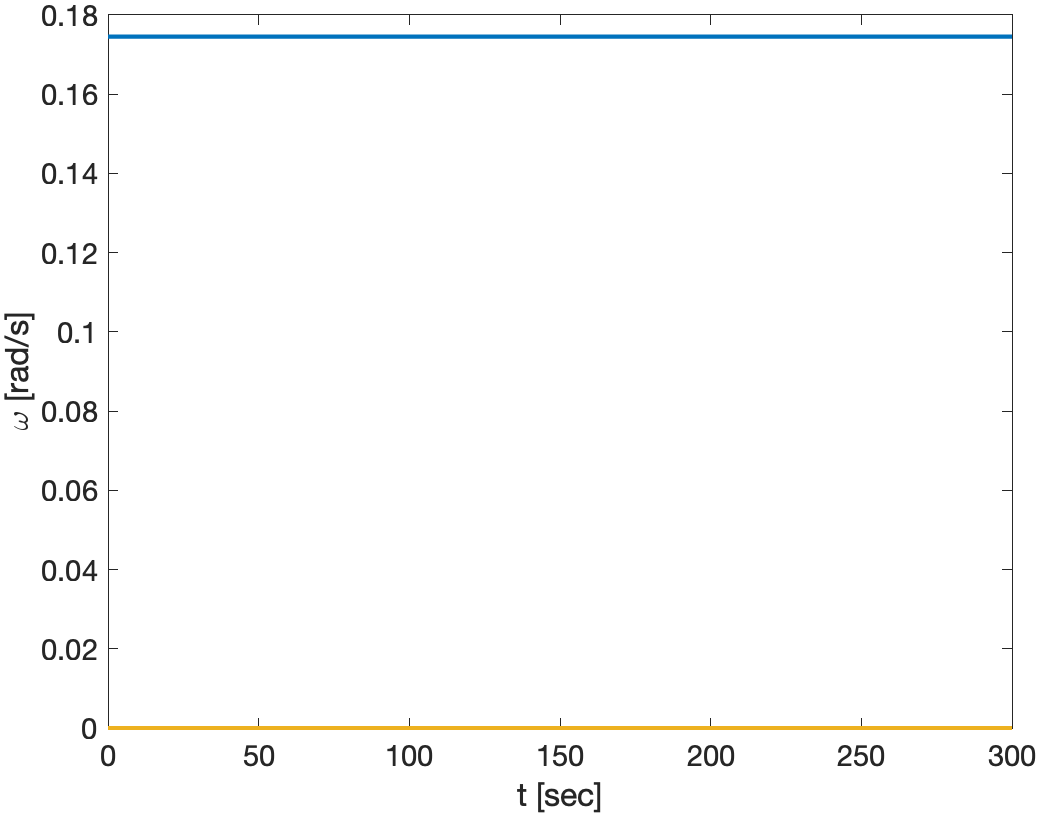
\includegraphics[width = 10cm]{Images/PS4/equilibrium_inertial_velocities.png}
    \caption{Angular Velocity Vector Components Expressed in the Principal Frame for Equilibrium about the Ineretial X-Axis}
    \label{fig:inertial_equilibrium_velocities}
\end{figure}

In Figure \ref{fig:inertial_equilibrium_velocities} it can be seen that the initial angular velocities are conserved for the full 300 second simulation. Primarily, $\omega_y$ and $\omega_z$ stay at zero.

\begin{figure}[H]
    \centering
    \captionsetup{justification = centering}
    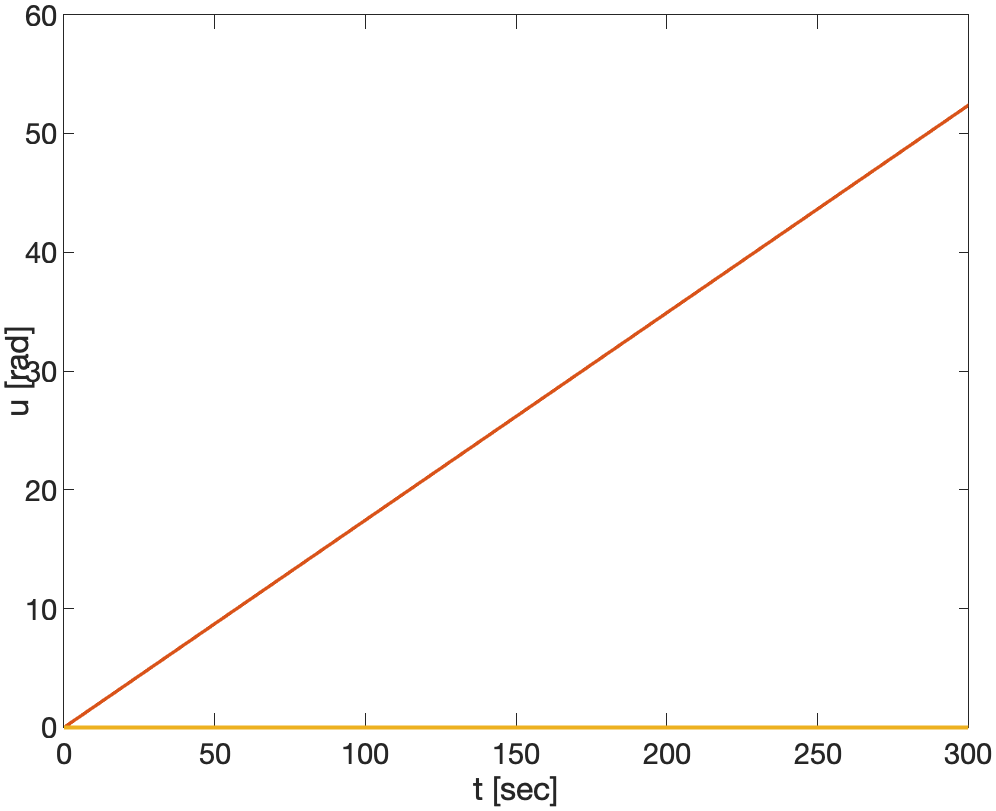
\includegraphics[width = 10cm]{Images/PS4/equilibrium_inertial_angles.png}
    \caption{312 Euler Angles Describing Rotation between Inertial and Principal Frame}
    \label{fig:inertial_equilibrium_angles}
\end{figure}

In Figure \ref{fig:inertial_equilibrium_angles}, it can be seen that $\psi$ and $\phi$ are zero for the full simulation and $\theta$ increases linearly which is consistent with the constant angular velocities.

\subsubsection{Repeat a. by setting the initial attitude to match the RTN frame. Set the initial angular velocity to
be non-zero only about N. Show the evolution of attitude motion in the RTN frame and give an
interpretation of the results (recall that you might have J2 effects in orbit propagation, consider
removing them for verification).}

To set the initial attitude to match the RTN frame, the initial position and velocity of the orbit was calculated in the ECI frame with the same orbital elements from Homework 2. From there the rotation matrix from ECI to RTN was found and then converted into Euler angles with the two functions shown below.

\begin{figure} [H]
    \centering
    \begin{lstlisting}
function u = RtoEuler312(R)

    u = zeros([3 1]);

    u(1) = atan2(R(1,2), R(2,2));
    u(2) = -asin(R(3,2));
    u(3) = atan2(R(3,1), R(3,3));

end

function R_eci_to_rtn = eci2rtn(r_eci, v_eci)
    
    % Compute radial, transverse, and normal vectors in ECI frame
    r_radial_eci = r_eci;
    r_normal_eci = cross(r_radial_eci, v_eci);
    r_transverse_eci = -cross(r_radial_eci, r_normal_eci);
    
    % Normalize radial, transverse, and normal vectors to obtain unit vectors
    r_radial_eci_unit = r_radial_eci / norm(r_radial_eci);
    r_transverse_eci_unit = r_transverse_eci / norm(r_transverse_eci);
    r_normal_eci_unit = r_normal_eci / norm(r_normal_eci);
    
    % Construct rotation matrix from ECI to RTN
    R_eci_to_rtn = [r_radial_eci_unit.'; r_transverse_eci_unit.'; r_normal_eci_unit.'];

end
    \end{lstlisting}
    \caption{Euler Angle RTN Alignment}
    \label{fig:euler_angle_prop_model}
\end{figure}

The simulink model from Homework 3 was then used to propagate the initial conditions with the only modification being that a simulink model was created to output the ECI to RTN DCM as the simulation was running as opposed to using a separate matlab script. This model is shown in Figures \ref{fig:orb_prop_simulink_num} and \ref{fig:orb_prop_simulink_kep} that show the two ways that the orbit could be propagated, Keplerian or Numerical methods.

\begin{figure}[H]
    \centering
    \captionsetup{ justification = centering}
    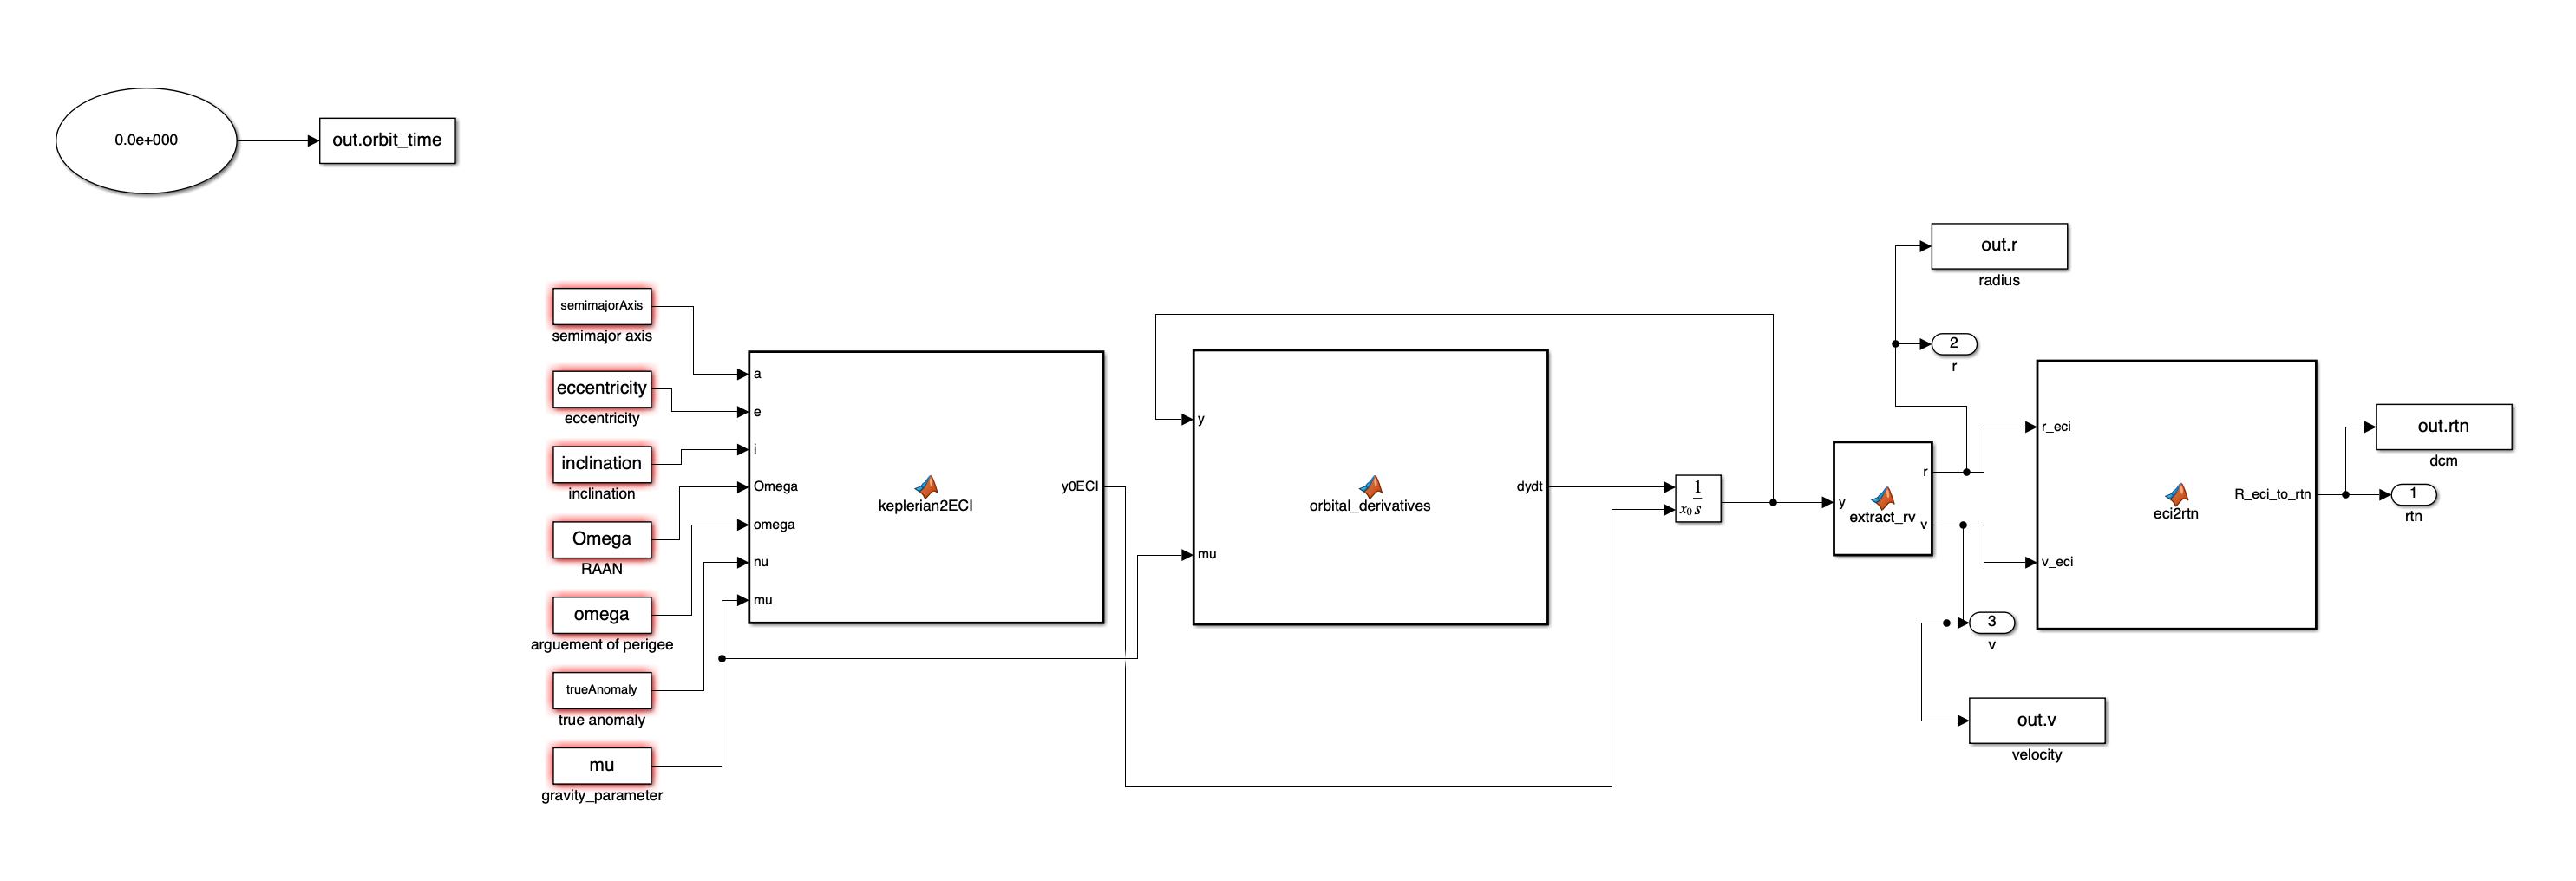
\includegraphics[width = 15cm]{Images/PS4/orbital_prop_simulink_num.png}
    \caption{Numerical Orbit Propagator Simulink Model}
    \label{fig:orb_prop_simulink_num}
\end{figure}

\begin{figure}[H]
    \centering
    \captionsetup{ justification = centering}
    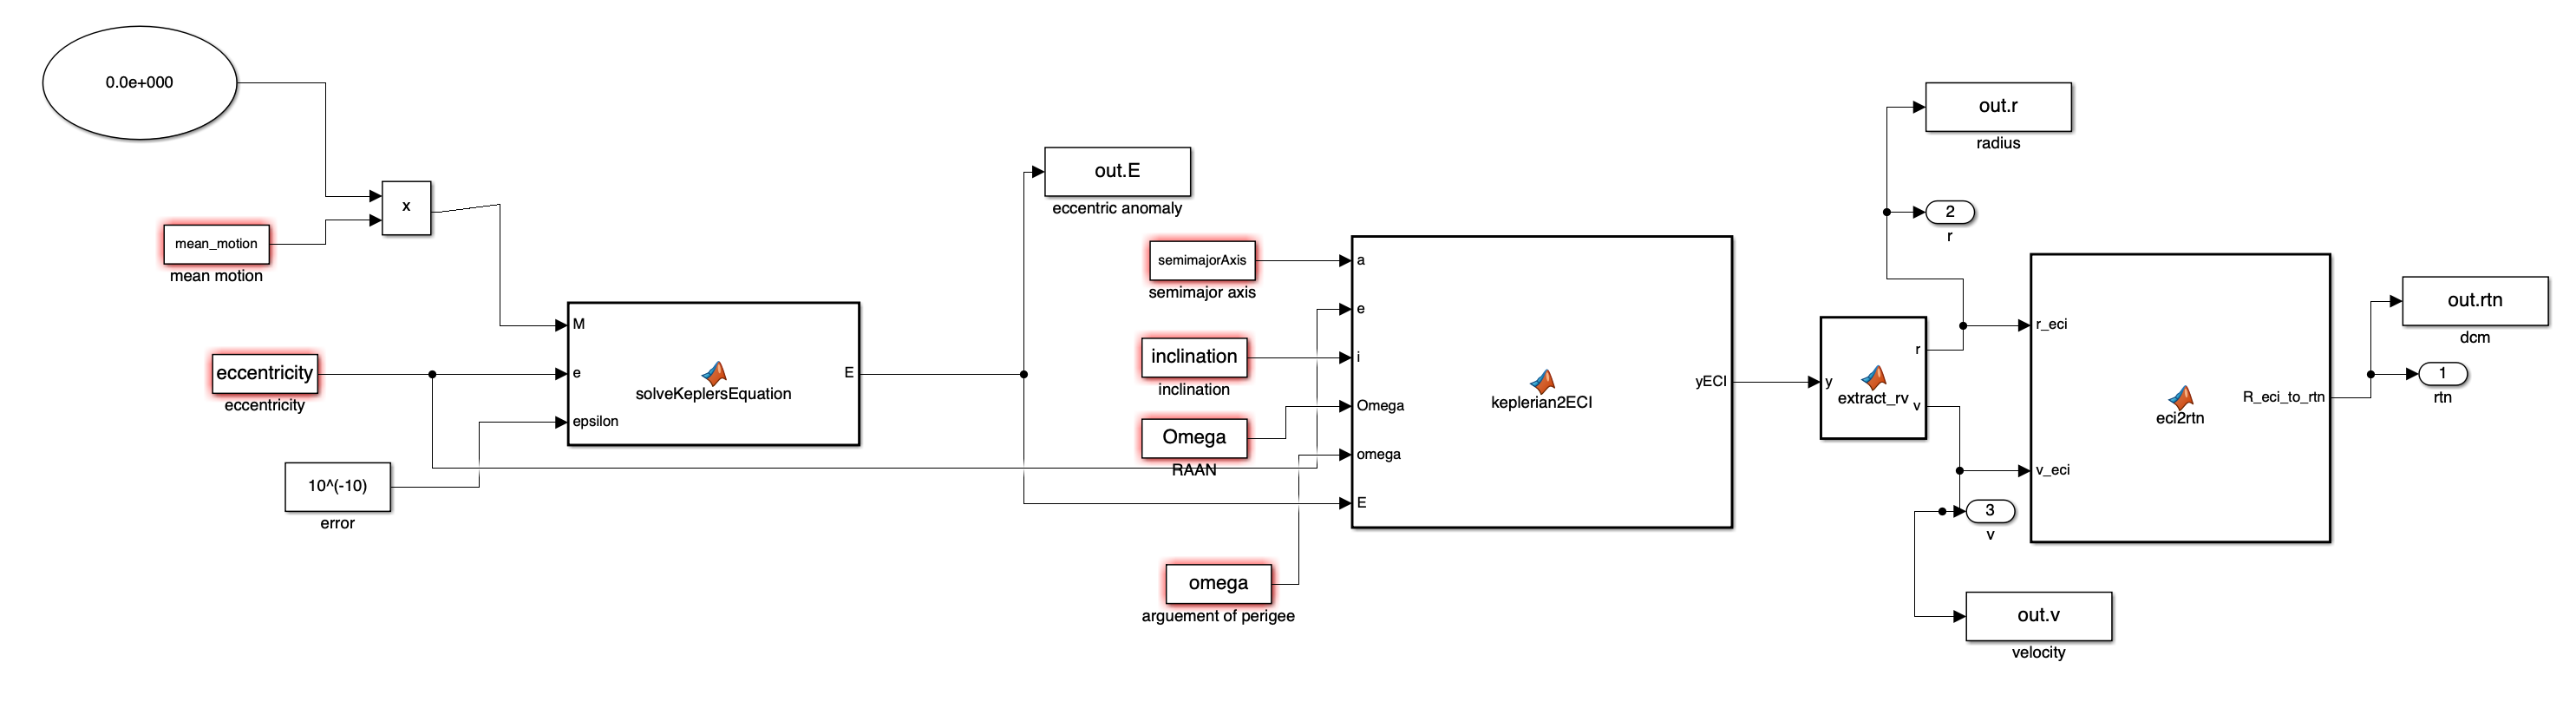
\includegraphics[width = 15cm]{Images/PS4/orbital_prop_simulink_kep.png}
    \caption{Keplerian Orbit Propagator Simulink Model}
    \label{fig:orb_prop_simulink_kep}
\end{figure}

Using this model, Figures \ref{fig:RTN_equilibrium_velocities} and \ref{fig:RTN_equilibrium_angles} were created.


\begin{figure}[H]
    \centering
    \captionsetup{ justification = centering}
    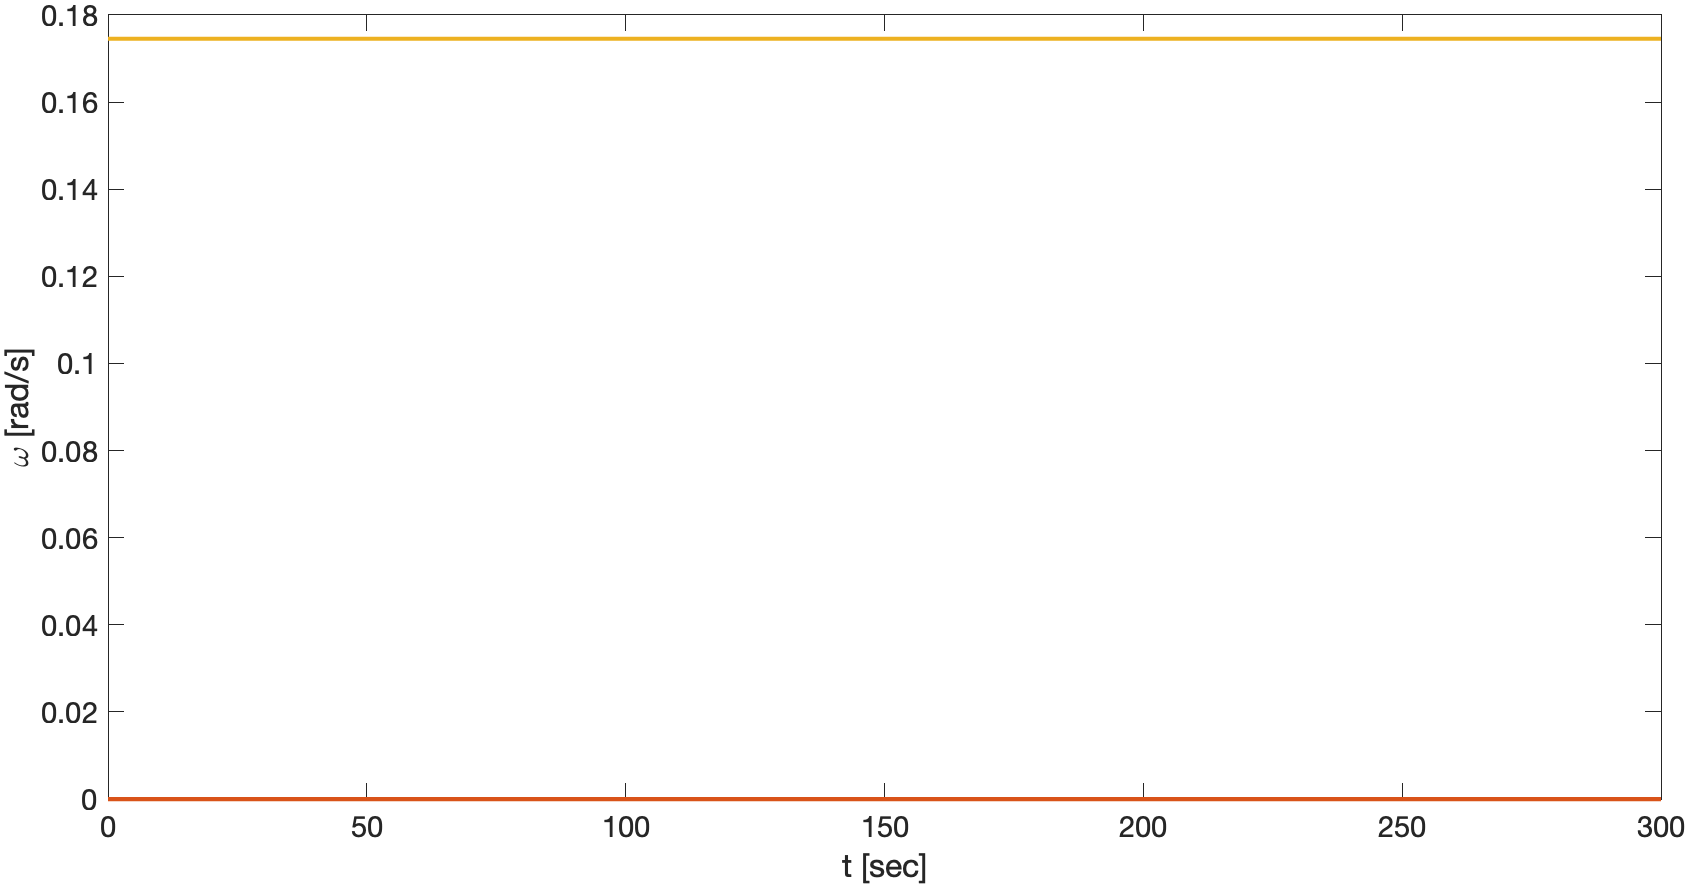
\includegraphics[width = 10cm]{Images/PS4/equilibrium_RTN_velocities.png}
    \caption{Angular Velocity Vector Components Expressed in the Principal Frame for Equilibrium about N-Axis}
    \label{fig:RTN_equilibrium_velocities}
\end{figure}

\begin{figure}[H]
    \centering
    \captionsetup{justification = centering}
    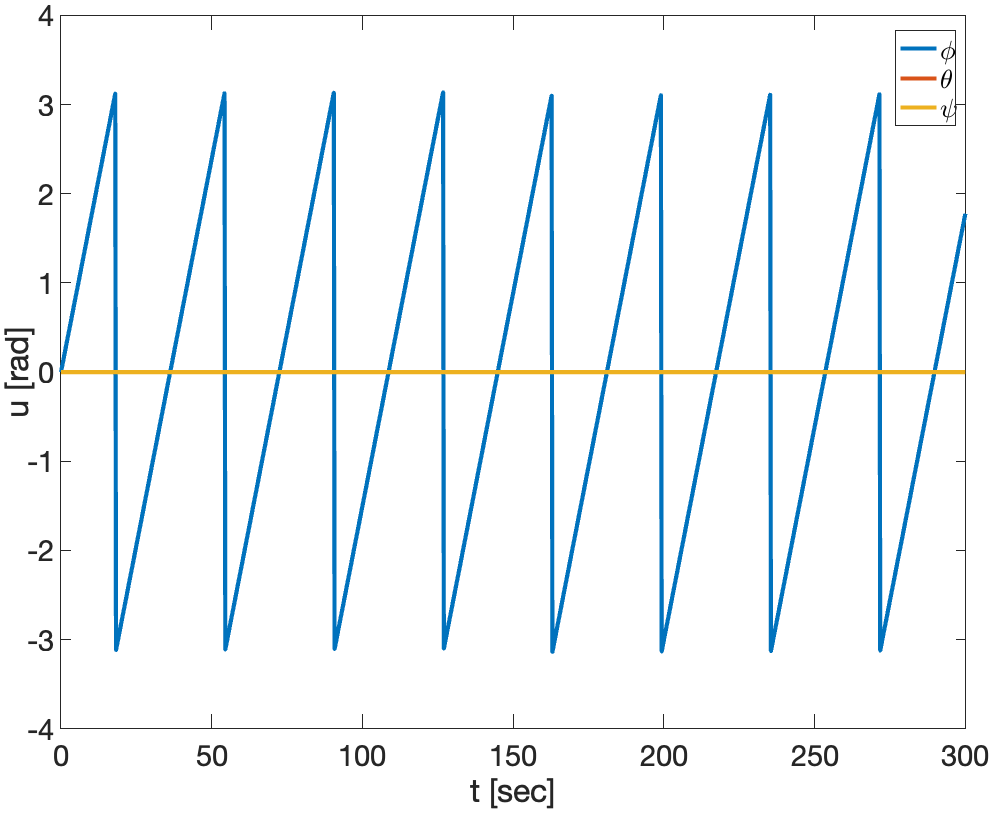
\includegraphics[width = 10cm]{Images/PS4/equilibrium_RTN_angles.png}
    \caption{312 Euler Angles Describing Rotation between RTN and Principal Frame}
    \label{fig:RTN_equilibrium_angles}
\end{figure}

In Figure \ref{fig:RTN_equilibrium_velocities} it can be seen that the angular velocities were once again constant, and in Figure \ref{fig:RTN_equilibrium_angles} it can be seen that the satellite only rotated about $\phi$ at a nearly constant rate (note that the maximum and minimum angles were capped at $\pi$ and $-\pi$). Due to the orbit of our satellite being almost circular, the radial vector's rate of change with respect to another frame doesn't change greatly throughout time. These results show that when the initial radial velocity is only in the N direction, it will stay at that velocity in equilibrium with Earth's gravitational field.

\subsection{Problem 2 - Stability Tests}

\subsubsection{Pretend you have a single-spin satellite. Set initial conditions to correspond alternatively to the 3
possible equilibrium configurations (rotation about principal axes of inertia). Slightly perturb initial
condition. Is the attitude stable or unstable? In angles and velocities? If stable, periodically or
asymptotically? Show it.}

To perturb the three possible equilibrium positions, the same simulation from Problem 1 was run three times while passing random numbers into the initial angular velocities and Euler angles. From this, Figures \ref{fig:stability_velocities} and \ref{fig:stability_angles} were created to shown the time histories of the perturbed angular velocities and Euler angles.

\begin{figure}[H]
    \centering
    \captionsetup{ justification = centering}
    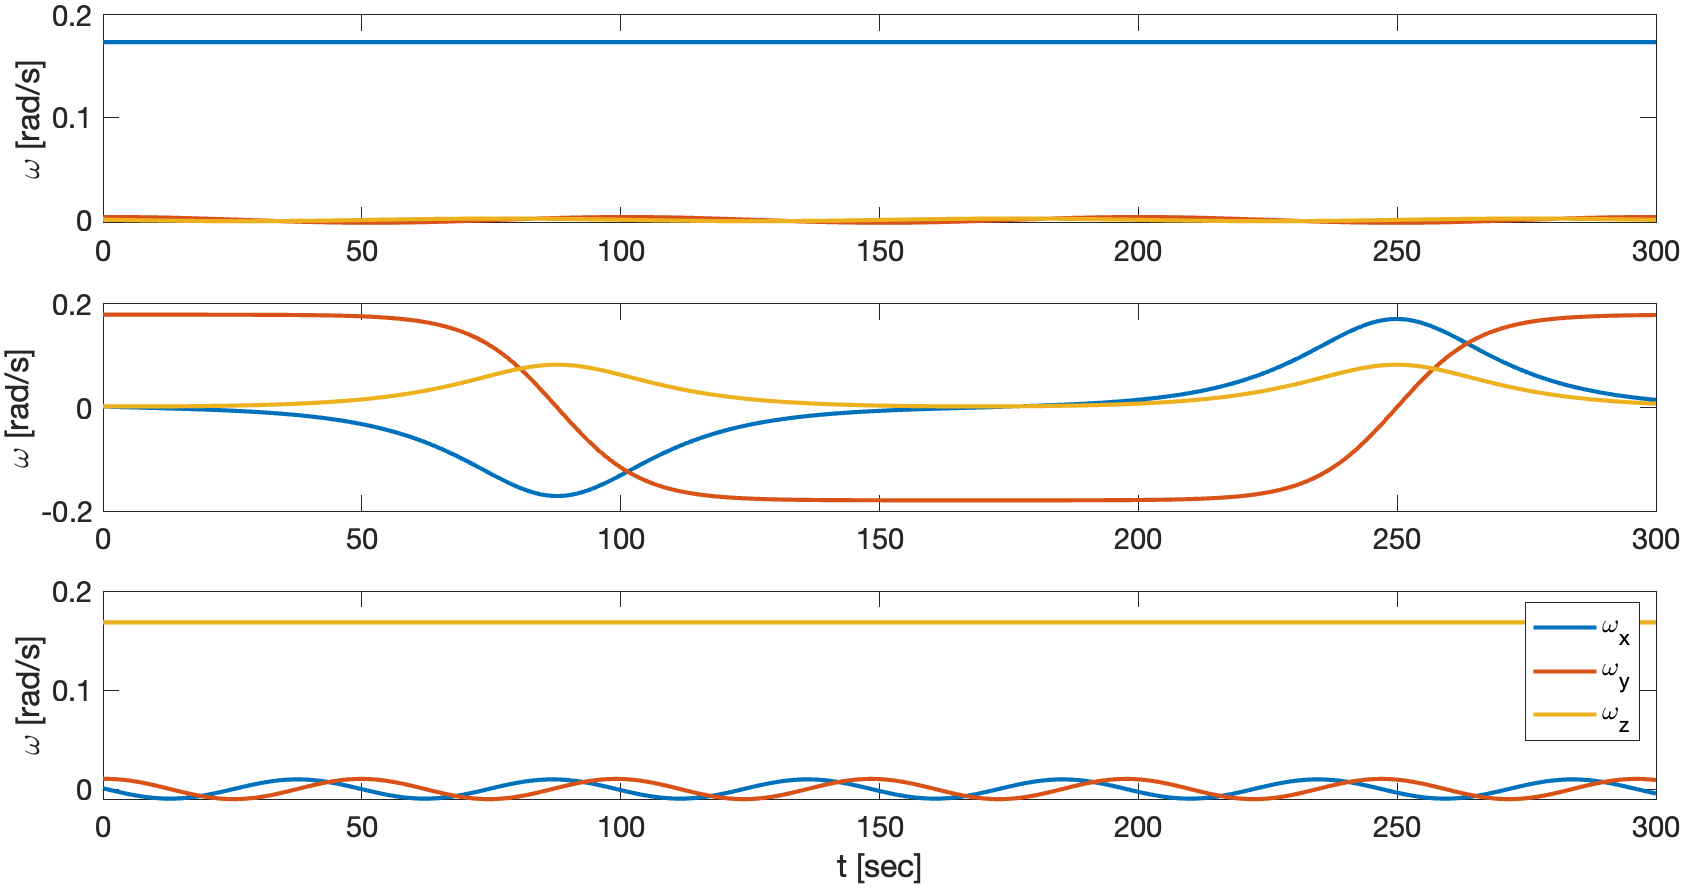
\includegraphics[width = 10cm]{Images/PS4/stability_history_velocity.png}
    \caption{Time History of Perturbed Angular Velocity Vector Components Expressed in Principal Frame}
    \label{fig:stability_velocities}
\end{figure}

\begin{figure}[H]
    \centering
    \captionsetup{justification = centering}
    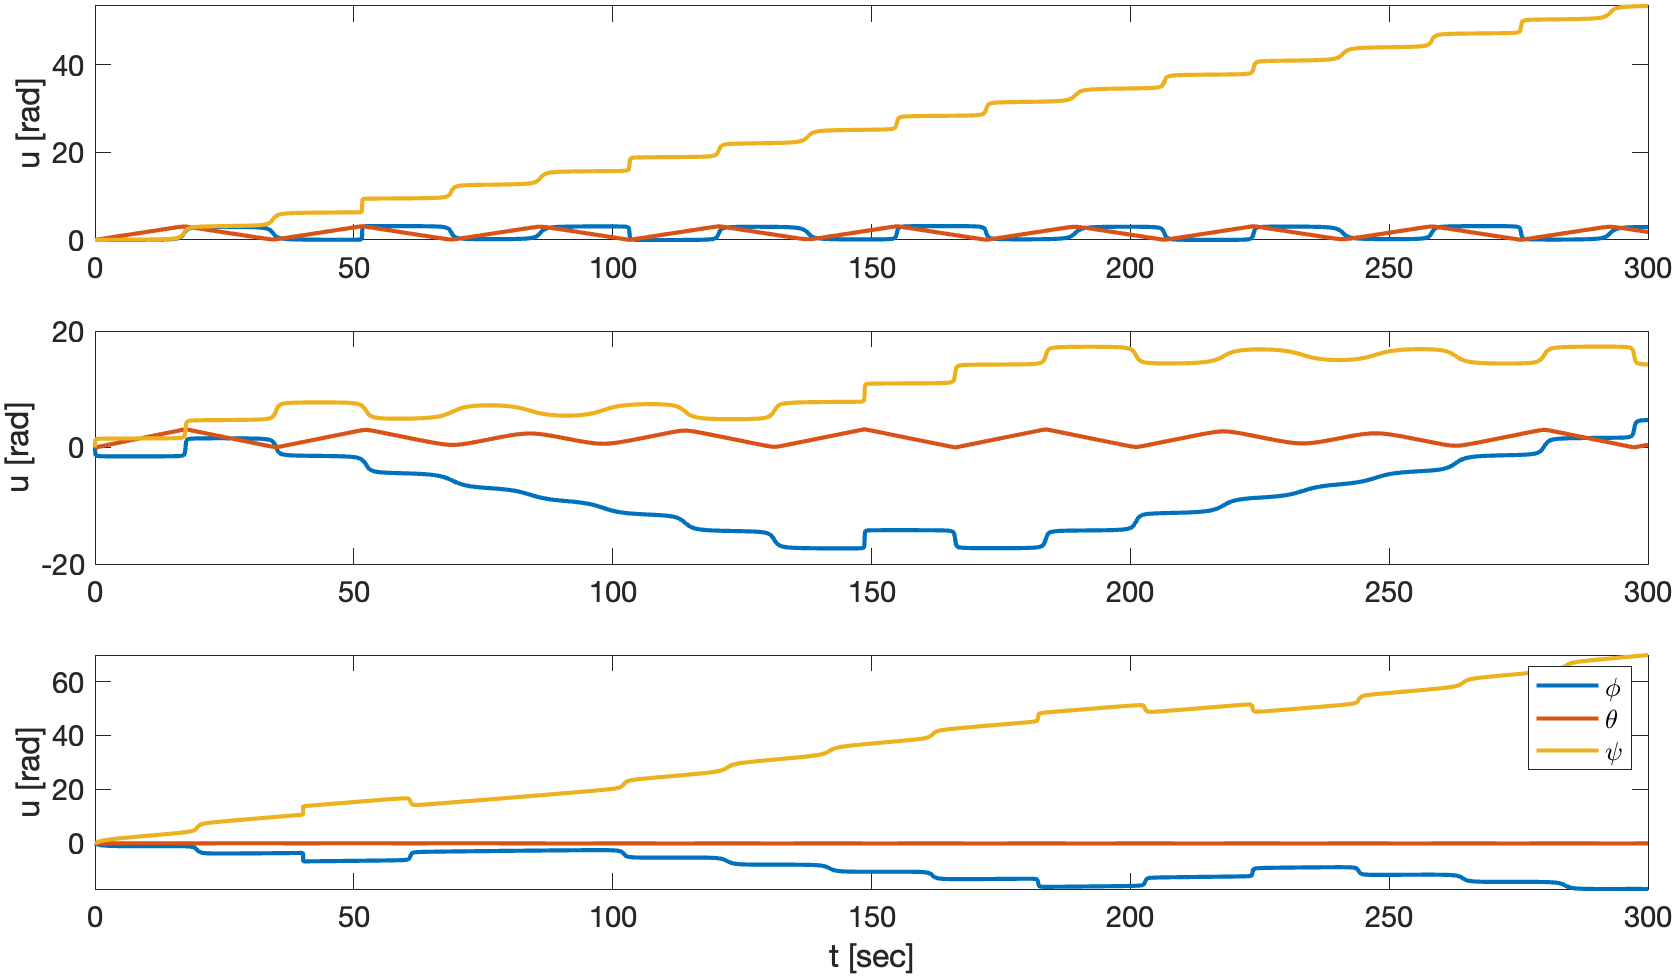
\includegraphics[width = 10cm]{Images/PS4/stability_history_angles.png}
    \caption{Time History of Perturbed 312 Euler Angles Describing Rotation between Inertial and Principal Frame}
    \label{fig:stability_angles}
\end{figure}

From these figures, it can be seen that when perturbing $\omega_x$ and $\omega_z$, the solutions were periodically stable. However, when perturbing $\omega_y$ the solutions were unstable and varied greatly across the simulation. This aligns with the theory supporting that asymptotic stability can be achieved for the maximum and minimum moments of inertia along the principle axes, but never the intermediate.

\subsection{Problem 3 - Adding a Momentum Wheel or Rotor (Dual-Spin Satellite)}

\subsubsection{Re-program Euler equations to include a generic momentum wheel or rotor with rotation axis
aligned with one of the principal axes of inertia. Ideally the wheel or rotor has specs representative
of commercial products (inertia, rotational speed).}

A momentum wheel was added to the Euler angle propagator through the simulink model shown below in Figure \ref{fig:dual_spin_simulink}. Additionally, the script used in the simulink model is shown below in Figure \ref{fig:dual_spin_simulink_code}.

\begin{figure} [H]
    \centering
    \captionsetup{justification = centering}
    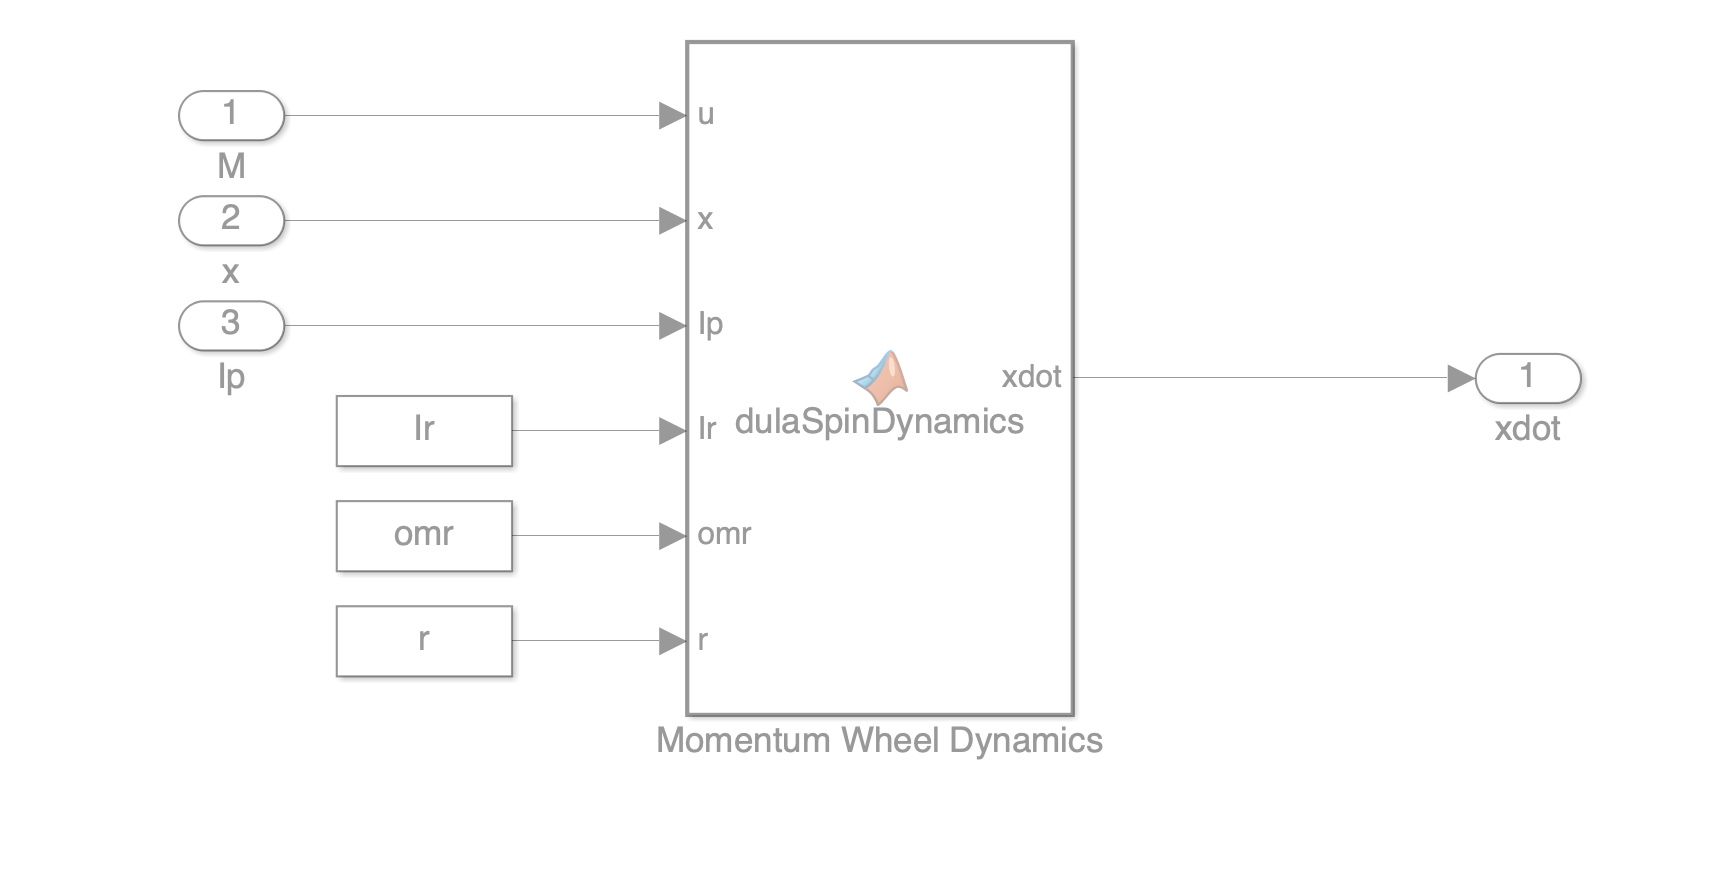
\includegraphics[width = 10cm]{Images/PS4/dualspin_simulink.png}
    \caption{Simulink Model to Account for Momentum Wheel in Euler Equations}
    \label{fig:dual_spin_simulink}
\end{figure}

\begin{figure} [H]
    \centering
    \begin{lstlisting}
function xdot = dualSpinDynamics(u,x,Ip,Ir,omr,r)

xdot = zeros(size(x));


Mx = u(1);
My = u(2);
Mz = u(3);

omx = x(1);
omy = x(2);
omz = x(3);

Ix = Ip(1,1);
Iy = Ip(2,2);
Iz = Ip(3,3);

rx = r(1);
ry = r(2);
rz = r(3);

wxdot = (1/Ix)*(Mx - ((Iz - Iy)*omy*omz + Ir*omr*(omy*rz - omz*ry)));
wydot = (1/Iy)*(My - ((Ix - Iz)*omz*omx + Ir*omr*(omz*rx - omx*rz)));
wzdot = (1/Iz)*(Mz - ((Iy - Ix)*omx*omy + Ir*omr*(omx*ry - omy*rx)));

xdot(1) = wxdot;
xdot(2) = wydot;
xdot(3) = wzdot;

end
    \end{lstlisting}
    \caption{Euler Angle Dual Spin Dynamics}
    \label{fig:dual_spin_simulink_code}
\end{figure}

\subsubsection{Numerically integrate Euler AND Kinematic equations from equilibrium initial condition. Verify
that integration is correct as from previous tests (conservation laws, rotations, etc.).}

To verify the integration, conservation of angular momentum was used. This was done by giving an initial angular velocity in all three of the inertial directions and plotting angular momentum to confirm that it remained constant throughout the integration. The results are shown below in Figure \ref{fig:mom_wheel_momentum_conservation}.

\begin{figure}[H]
    \centering
    \captionsetup{justification = centering}
    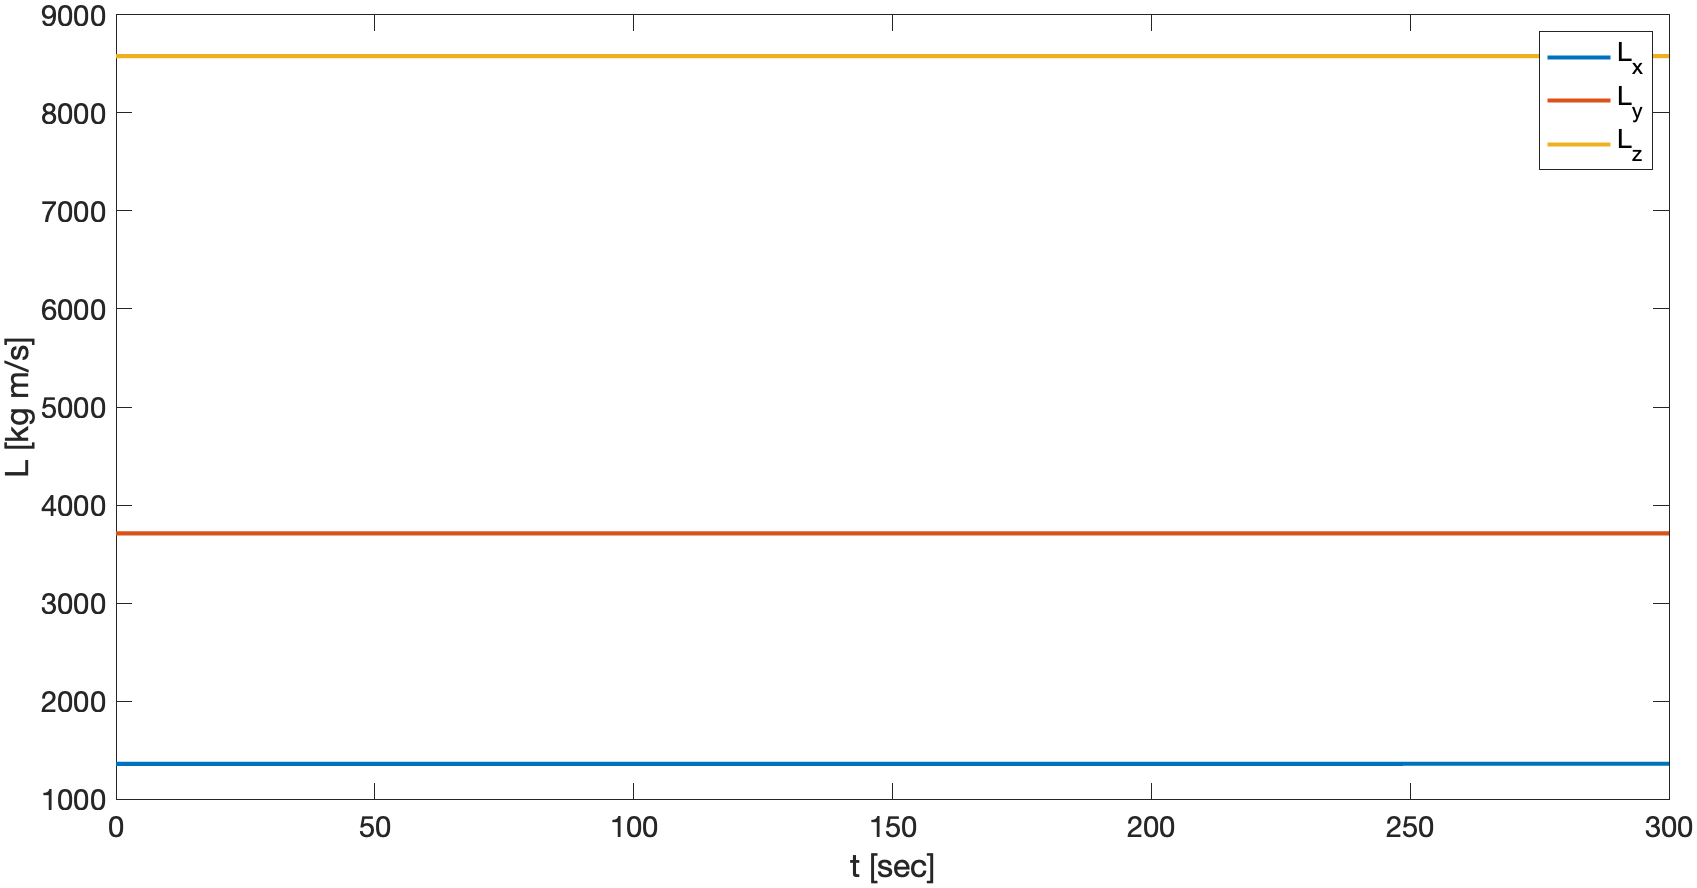
\includegraphics[width = 10cm]{Images/mom_wheel_angular_momentum.png}
    \caption{Angular Momentum Vector Components Represented in the Inertial Frame Plotted over Time}
    \label{fig:mom_wheel_momentum_conservation}
\end{figure}

In Figure \ref{fig:mom_wheel_momentum_conservation}, it can be seen that angular momentum was conserved in all three of the inertial directions, thus validating the new integration scheme for the momentum wheel.

\subsubsection{Verify equilibrium and its stability similar to previous pset.}

Just like in problem 1, the initial Euler angles were first aligned with the inertial frame to obtain results shown in Figures \ref{fig:mom_wheel_inertial_equilibrium} and \ref{fig:mom_wheel_equilibrium_inertial_angles}.

\begin{figure}[H]
    \centering
    \captionsetup{justification = centering}
    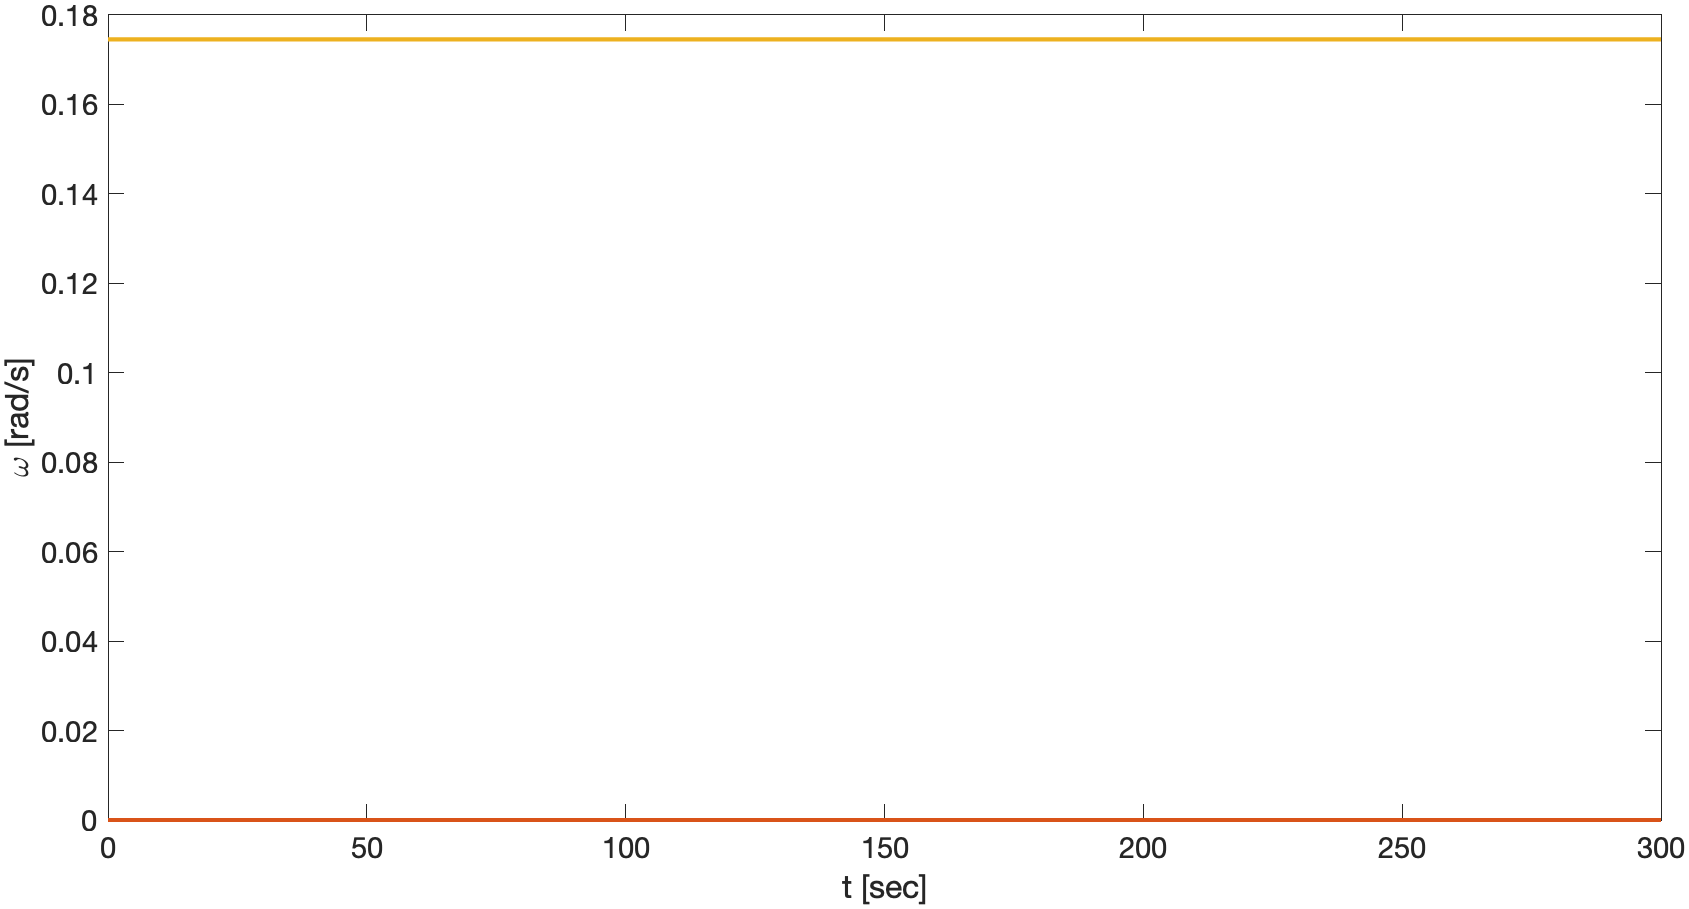
\includegraphics[width = 10cm]{Images/PS4/mom_wheel_equilibrium_inertial_velocities.png}
    \caption{Angular Velocity Vector Components Expressed in the Principal Frame for Equilibrium about the Inertial Z-Axis}
    \label{fig:mom_wheel_inertial_equilibrium}
\end{figure}

\begin{figure}[H]
    \centering
    \captionsetup{justification = centering}
    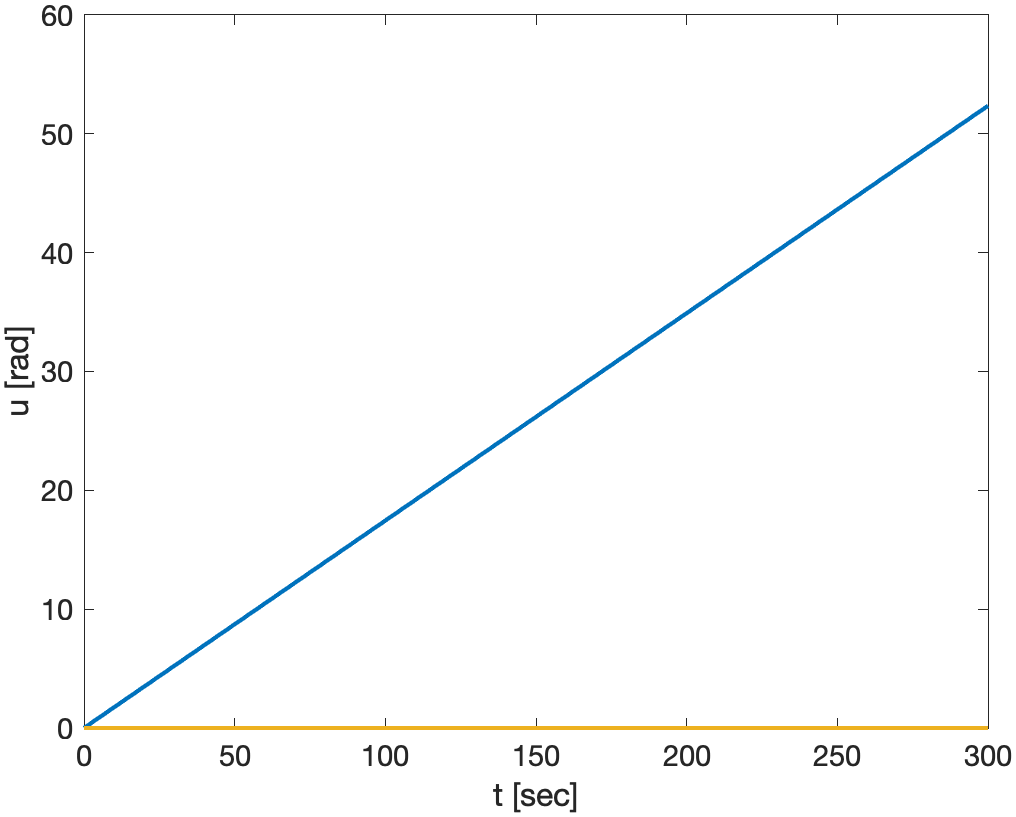
\includegraphics[width = 10cm]{Images/PS4/mom_wheel_equilibrium_inertial_angles.png}
    \caption{312 Euler Angles Describing Rotation between Inertial and Principal Frame}
    \label{fig:mom_wheel_equilibrium_inertial_angles}
\end{figure}

Figures \ref{fig:mom_wheel_inertial_equilibrium} and \ref{fig:mom_wheel_equilibrium_inertial_angles} show that once again the angular velocity vector components remained constant and the rotation between the inertial and principal frames only happened in one direction.

Next, the initial Euler angles were aligned with the RTN frame through the same procedure shown in problem 1 to obtain Figures \ref{fig:mom_wheel_RTN_equilibrium} and \ref{fig:mom_wheel_equilibrium_RTN_angles}.

\begin{figure}[H]
    \centering
    \captionsetup{justification = centering}
    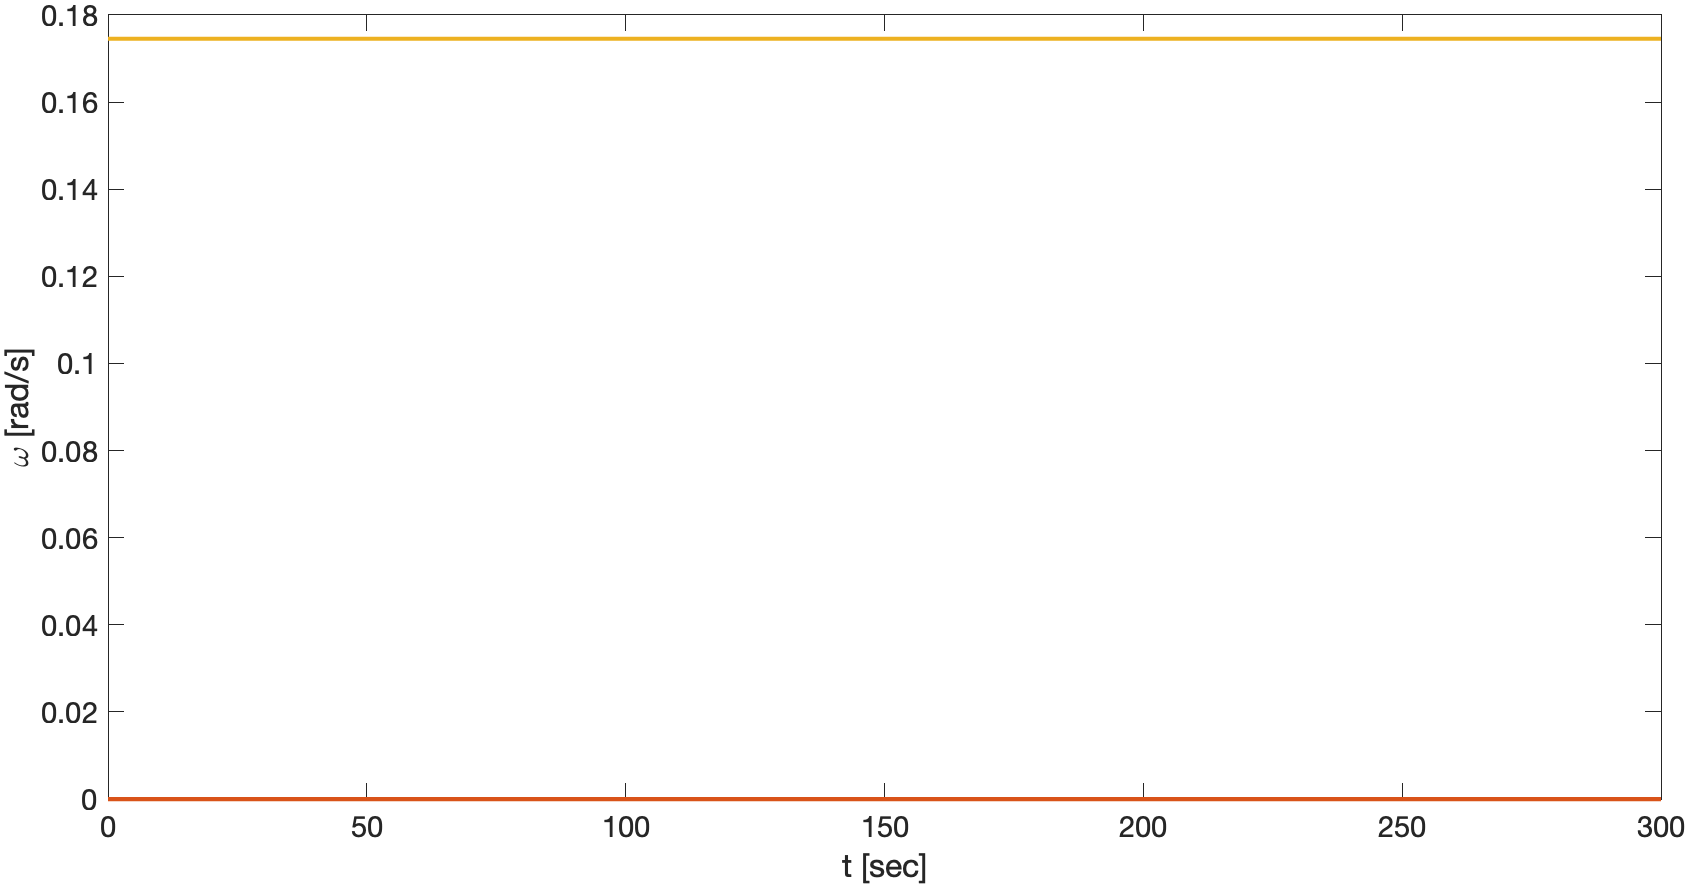
\includegraphics[width = 10cm]{Images/PS4/mom_wheel_equilibrium_RTN_velocities.png}
    \caption{Angular Velocity Vector Components Expressed in the Principal Frame for Equilibrium about the N-Axis}
    \label{fig:mom_wheel_RTN_equilibrium}
\end{figure}

\begin{figure}[H]
    \centering
    \captionsetup{justification = centering}
    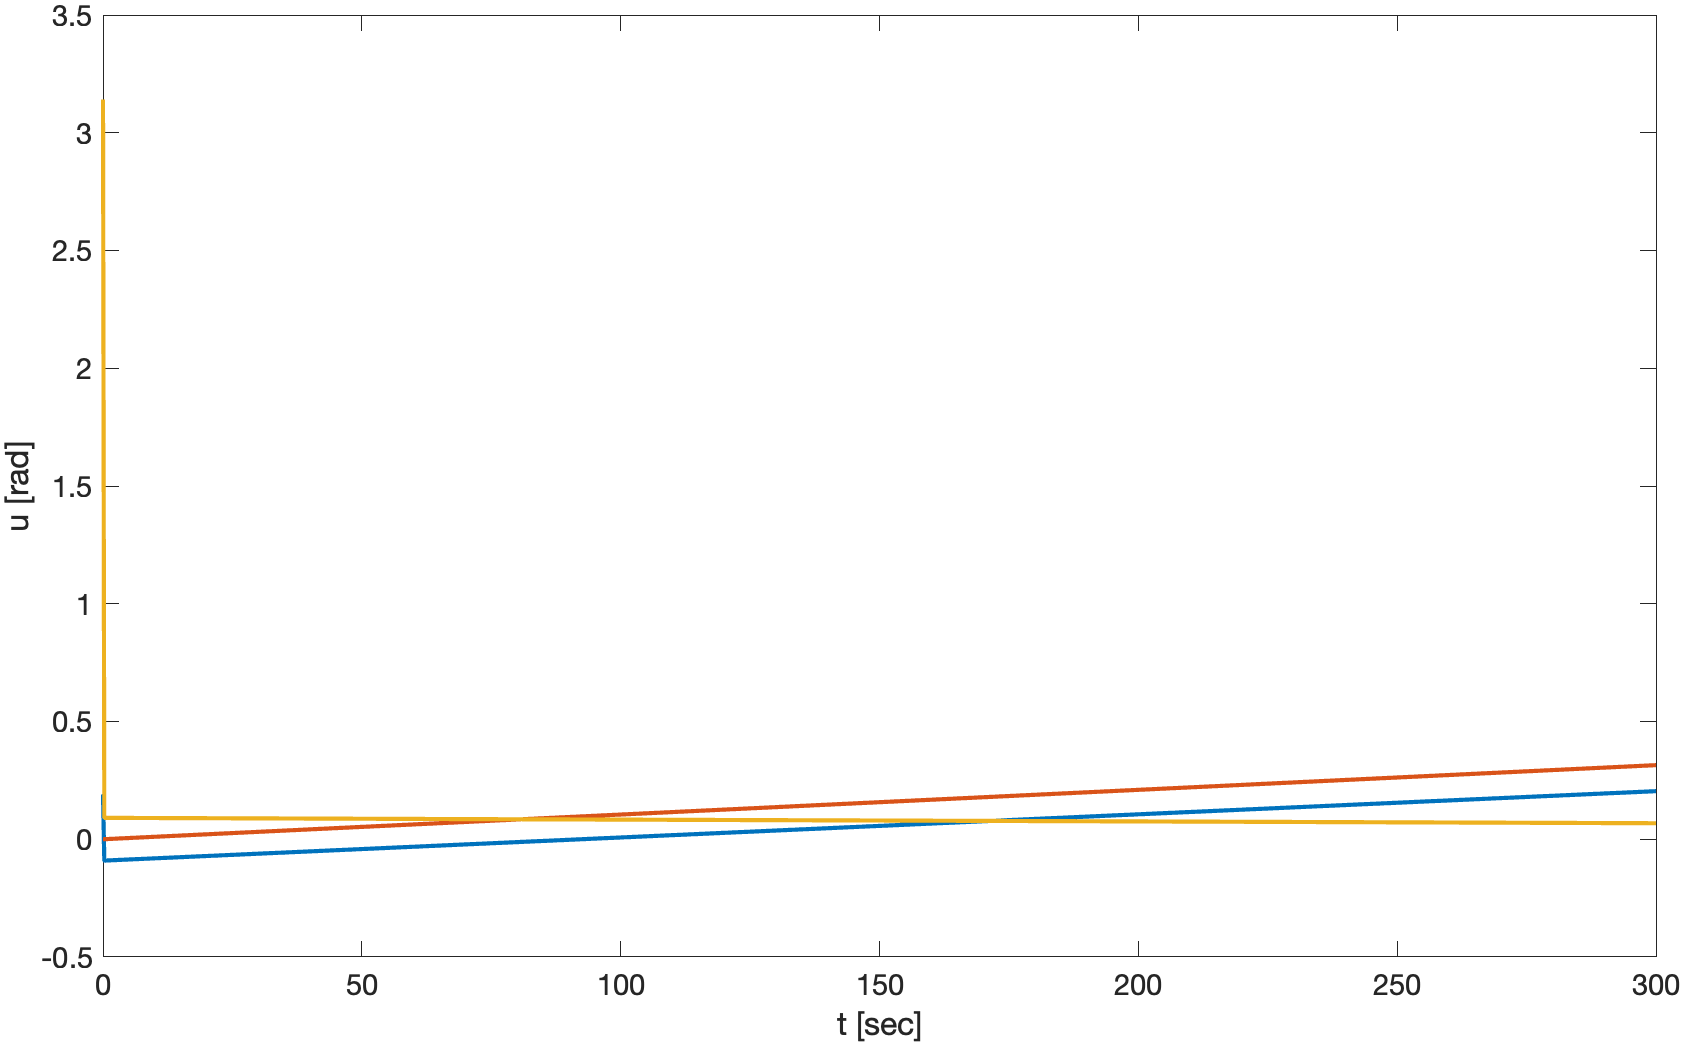
\includegraphics[width = 10cm]{Images/PS4/mom_wheel_equilibrium_RTN_angles.png}
    \caption{312 Euler Angles Describing Rotation between Inertial and Principal Frame}
    \label{fig:mom_wheel_equilibrium_RTN_angles}
\end{figure}

Figures \ref{fig:mom_wheel_RTN_equilibrium} and \ref{fig:mom_wheel_equilibrium_RTN_angles} show that equilibrium about the N-Axis was once again achieved through having zero angular velocity in the other two directions. Additionally, the Euler angles only rotated in one direction between the two frames.

The same procedure of using random initial conditions was used for the momentum stability test. Through selecting random initial conditions for the Euler angles and angular velocities, Figures \ref{fig:mom_wheel_stability_velocities} and \ref{fig:mom_wheel_stability_angles} were created.

\begin{figure}[H]
    \centering
    \captionsetup{ justification = centering}
    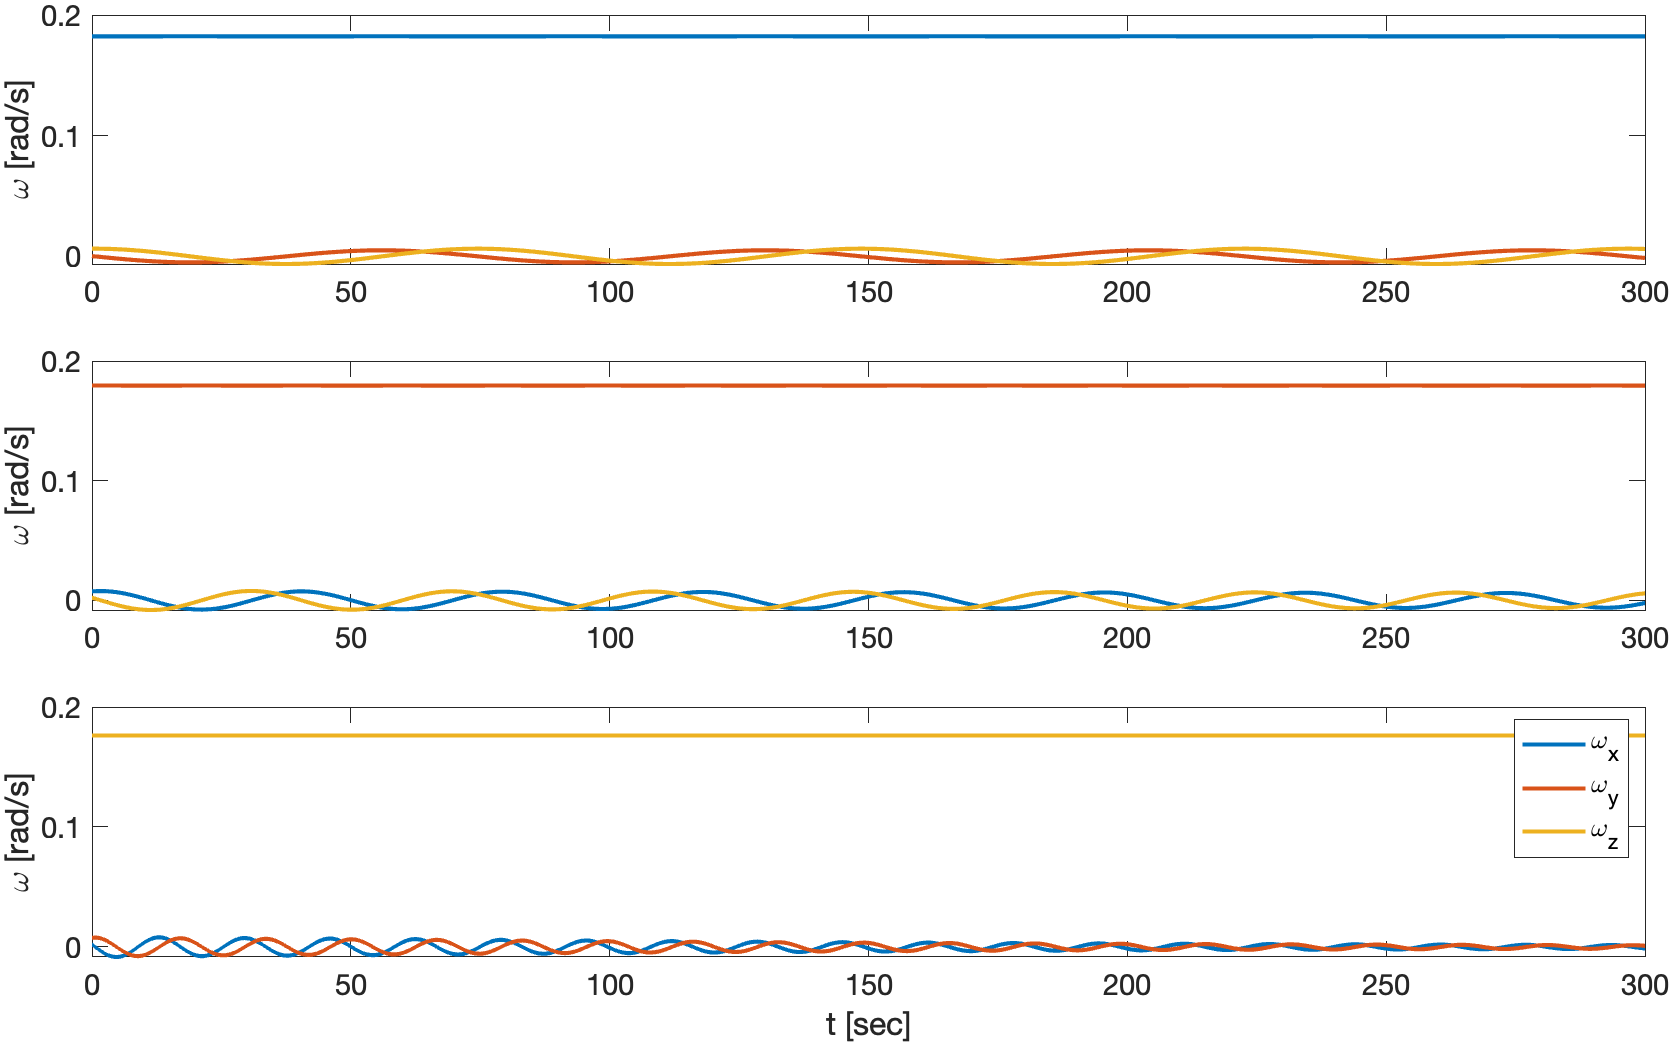
\includegraphics[width = 10cm]{Images/PS4/mom_wheel_stability_history_velocity.png}
    \caption{Time History of Perturbed Angular Velocity Vector Components Expressed in Principal Frame}
    \label{fig:mom_wheel_stability_velocities}
\end{figure}

\begin{figure}[H]
    \centering
    \captionsetup{justification = centering}
    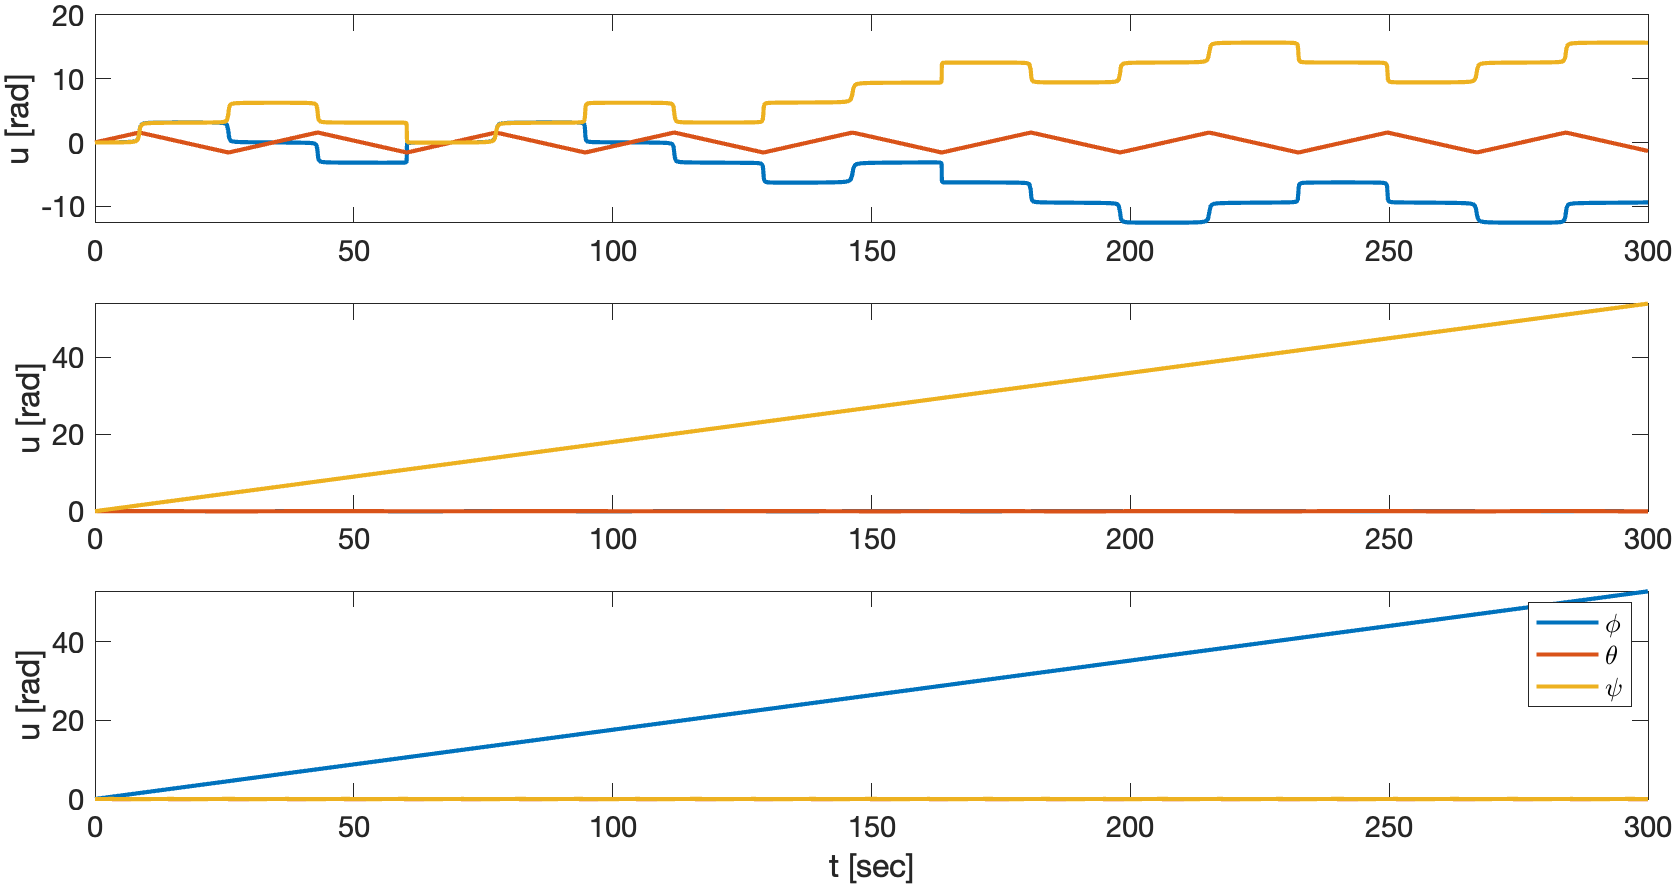
\includegraphics[width = 10cm]{Images/PS4/mom_wheel_stability_history_angles.png}
    \caption{Time History of Perturbed 312 Euler Angles Describing Rotation between Inertial and Principal Frame}
    \label{fig:mom_wheel_stability_angles}
\end{figure}

Figures \ref{fig:mom_wheel_stability_velocities} and \ref{fig:mom_wheel_stability_angles} show that once again, the angular velocities and Euler angles were stable in two of the three axes. 

\subsubsection{Use the stability condition to make attitude motion stable for rotation about intermediate moment of inertia by changing moment of inertia and/or angular velocity of the momentum wheel or rotor.}



\begin{figure}[H]
    \centering
    \captionsetup{ justification = centering}
    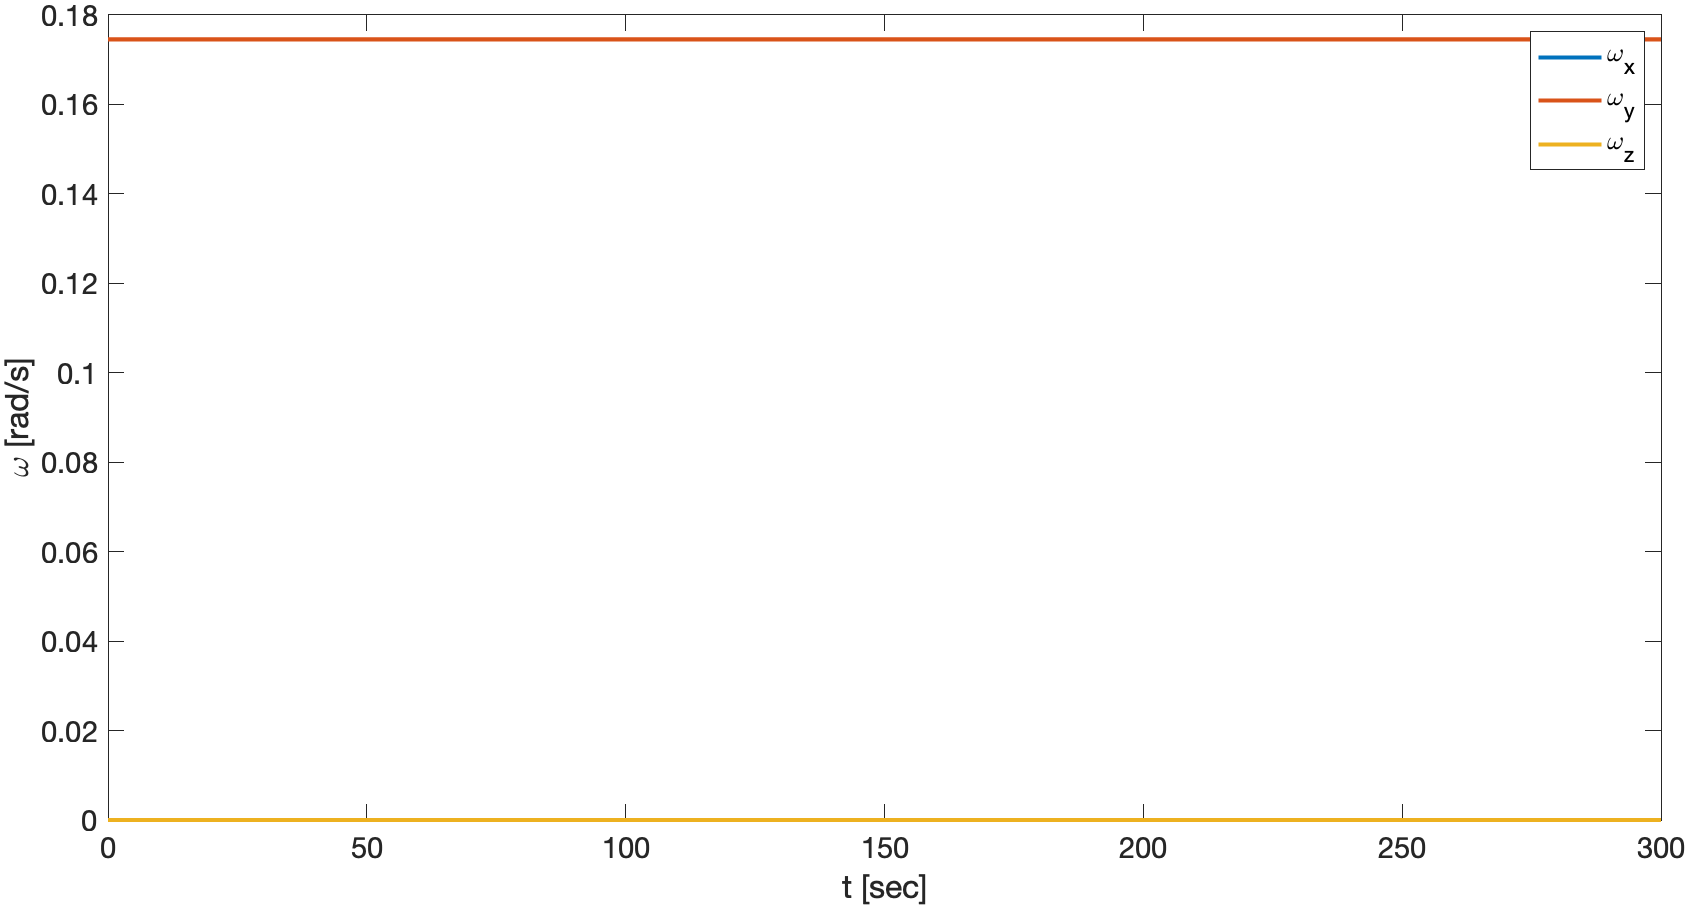
\includegraphics[width = 10cm]{Images/PS4/mom_wheel_intermediate_stability_history_velocity.png}
    \caption{Time History of Perturbed Angular Velocity Vector Components Expressed in Principal Frame}
    \label{fig:mom_wheel_intermediate_stability_velocities}
\end{figure}

\begin{figure}[H]
    \centering
    \captionsetup{justification = centering}
    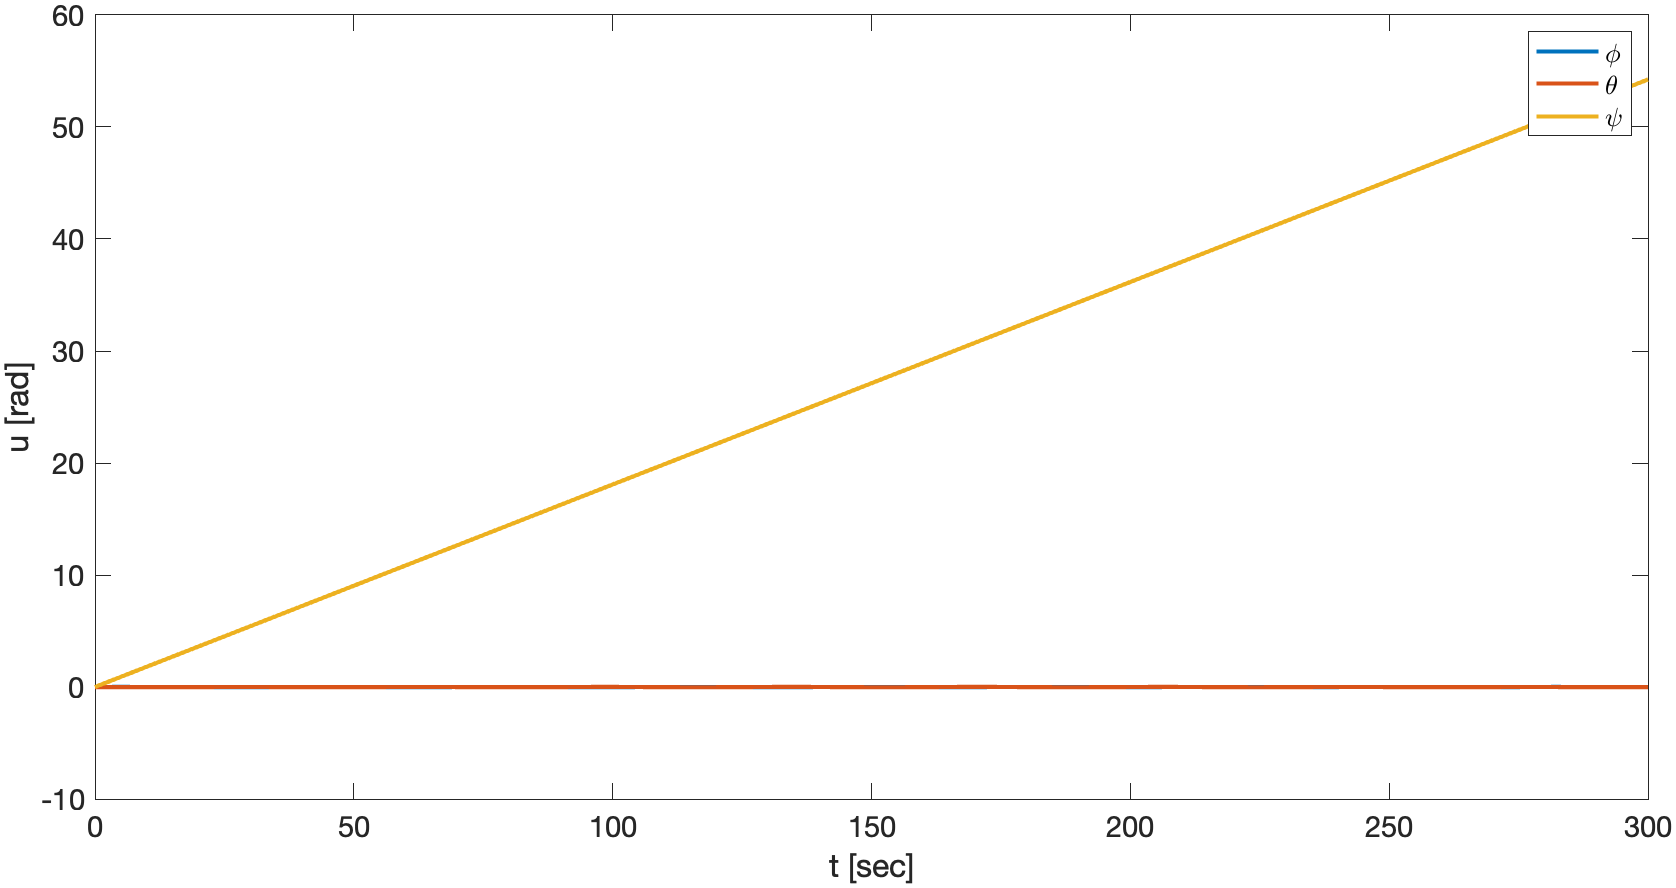
\includegraphics[width = 10cm]{Images/PS4/mom_wheel_intermediate_stability_history_angles.png}
    \caption{Time History of Perturbed 312 Euler Angles Describing Rotation between Inertial and Principal Frame}
    \label{fig:mom_wheel_inermediate_stability_angles}
\end{figure}

\subsubsection{Try to make rotation about another arbitrary axis (potentially relevant to your project) stable
through a generic momentum wheel or rotor.}

\begin{figure}[H]
    \centering
    \captionsetup{ justification = centering}
    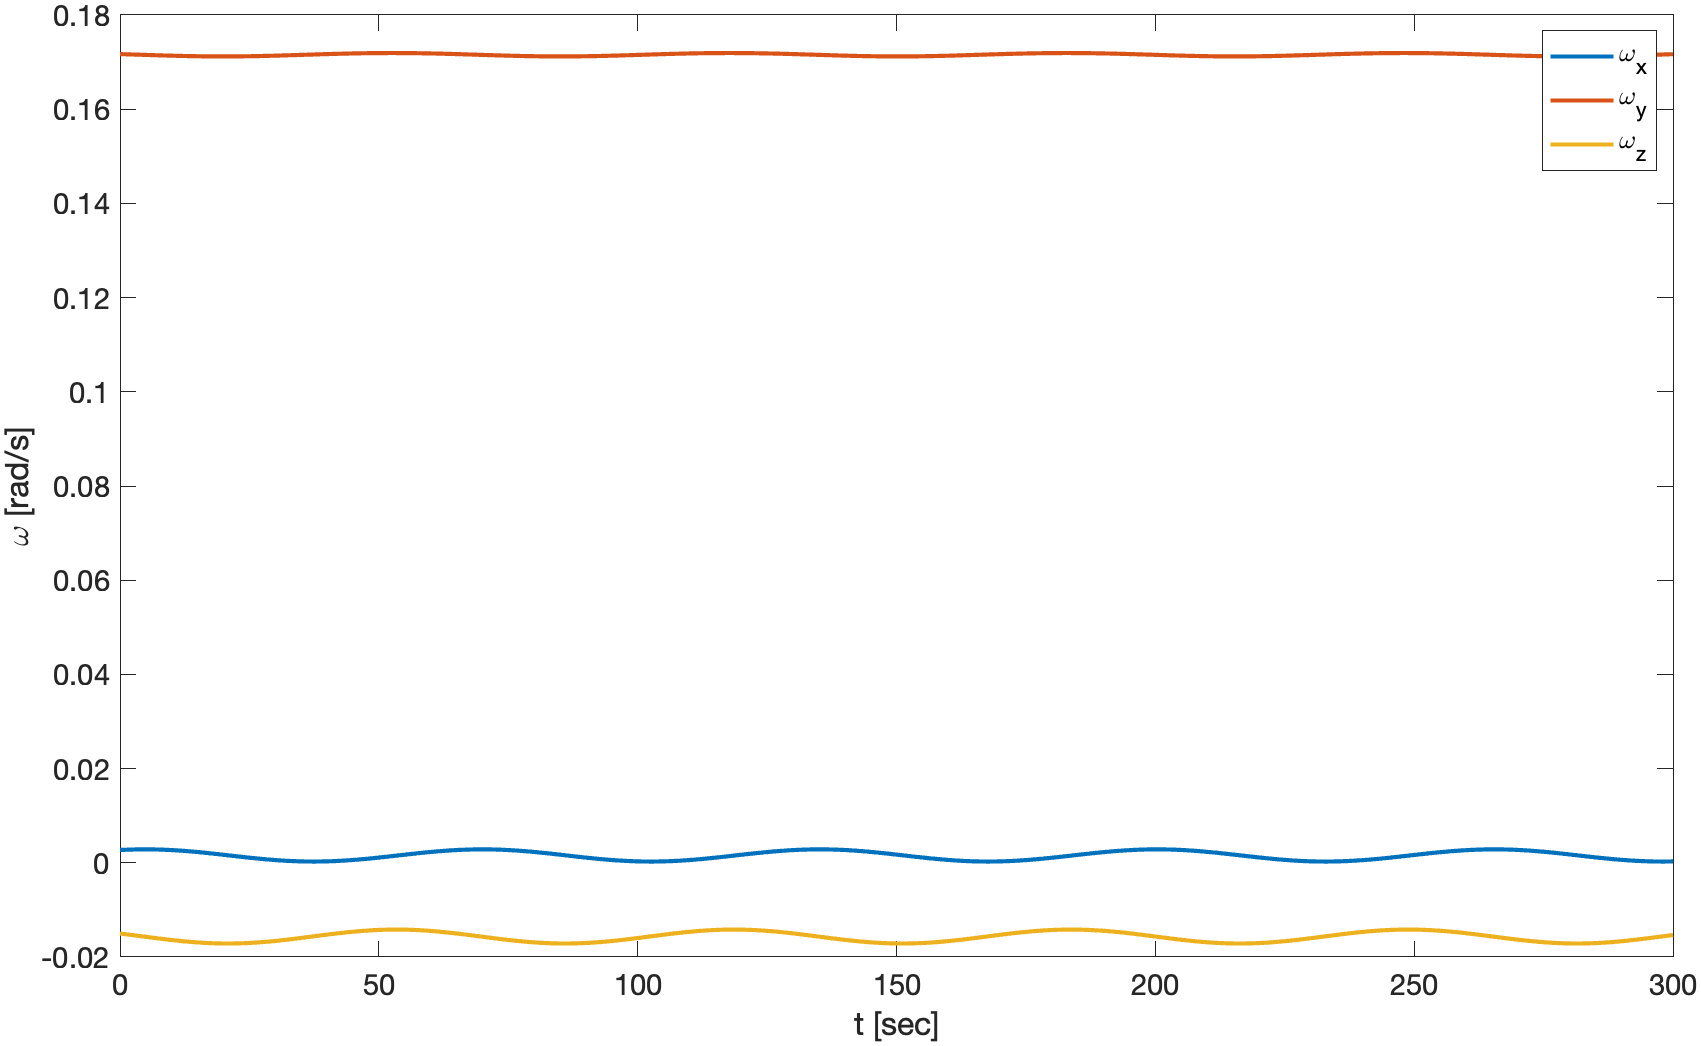
\includegraphics[width = 10cm]{Images/PS4/mom_wheel_mission_stability_history_velocity.png}
    \caption{Time History of Perturbed Angular Velocity Vector Components Expressed in Principal Frame}
    \label{fig:mom_wheel_mission_stability_velocities}
\end{figure}

\begin{figure}[H]
    \centering
    \captionsetup{justification = centering}
    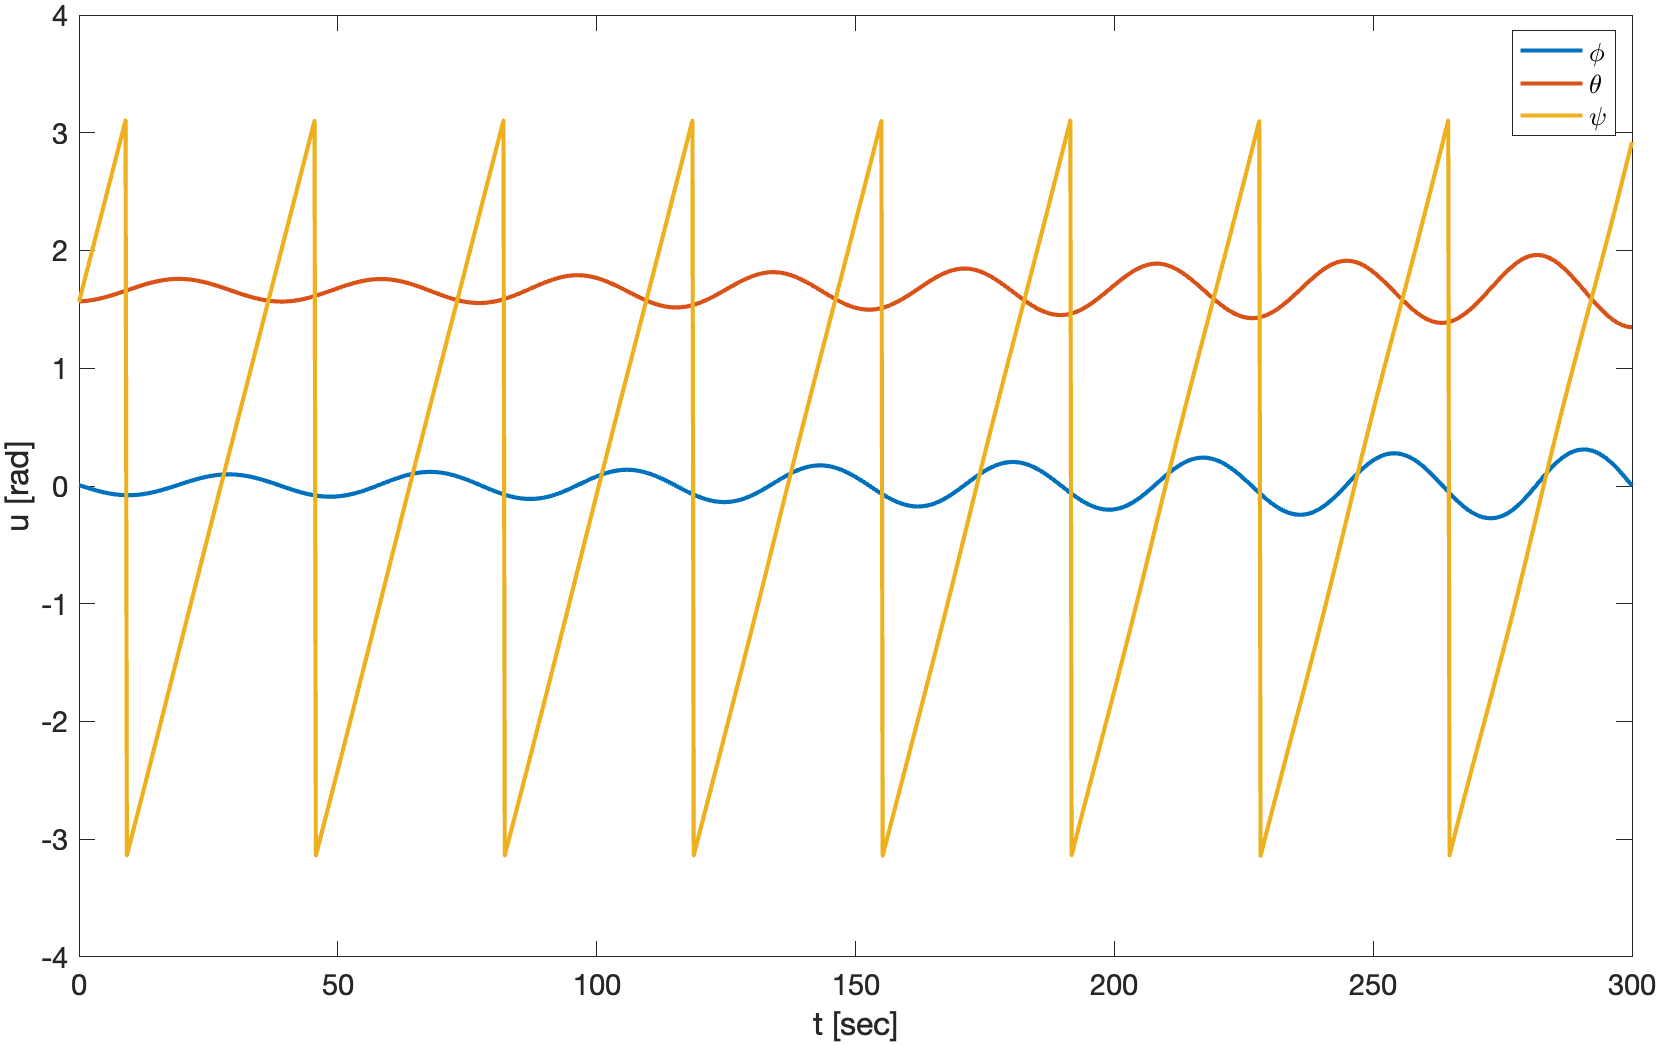
\includegraphics[width = 10cm]{Images/PS4/mom_wheel_mission_stability_history_angles.png}
    \caption{Time History of Perturbed 313 Euler Angles Describing Rotation between Inertial and Body Frame}
    \label{fig:mom_wheel_mission_stability_angles}
\end{figure}

\subsection{Problem 4 - Gravity Gradient Torque (Modeling)}

\subsubsection{Remove rotor.}

The simulink model created for this uses variant subsystems to switch between the single and dual rotation configurations very easily.

\subsubsection{Program gravity gradient torque. Feed torque to Euler equations. This is the first perturbation you
model resulting from the interaction of the spacecraft with the environment. Hint: change your orbit
to make gravity gradient significant if that’s not the case.}

\begin{figure}[H]
    \centering
    \captionsetup{justification = centering}
    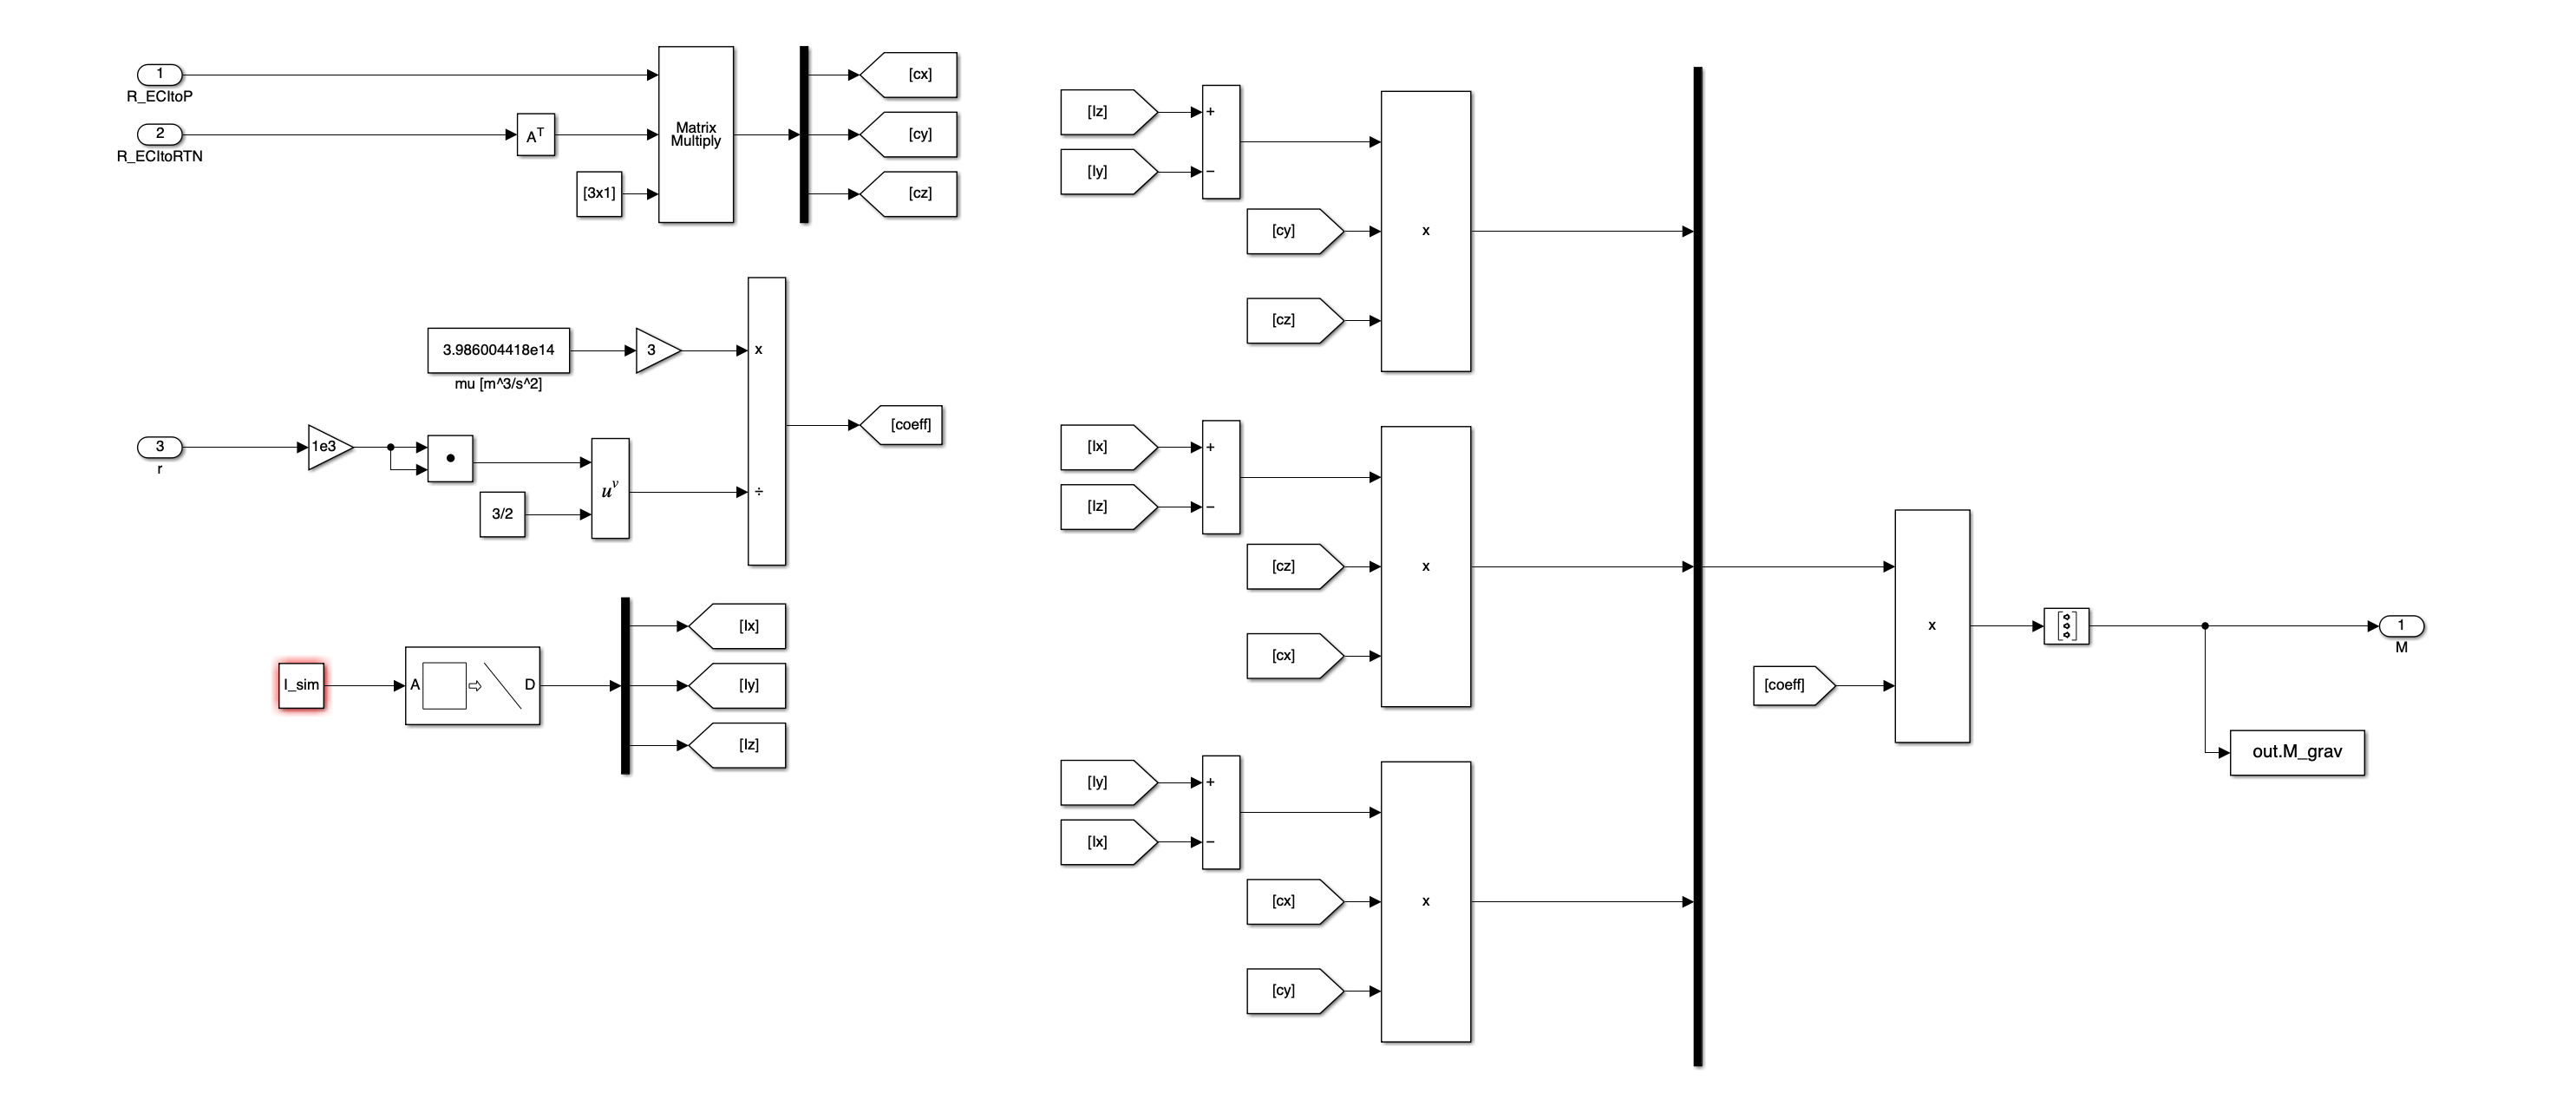
\includegraphics[width = 15cm]{Images/PS4/gravity_gradiant_simulink_model.png}
    \caption{Simulink Model for Gravity Gradient Perturbation}
    \label{fig:grav_gradient_simulink}
\end{figure}

\subsubsection{Verify that the magnitude of the modelled torque is consistent with the orbit and inertia tensor of
your satellite. Hint: use simplified formulas from class on modelling of gravity gradient torque.}

\subsubsection{Numerically integrate Euler and Kinematic equations including gravity gradient from initial
conditions corresponding to body axes aligned with the orbital frame (RTN). Verify that gravity
gradient torque is zero, besides numerical errors. Hint: you may need to simplify the orbit to
unperturbed circular to achieve this. Check that initial angular velocity matches mean motion.}

\begin{figure}[H]
    \centering
    \captionsetup{ justification = centering}
    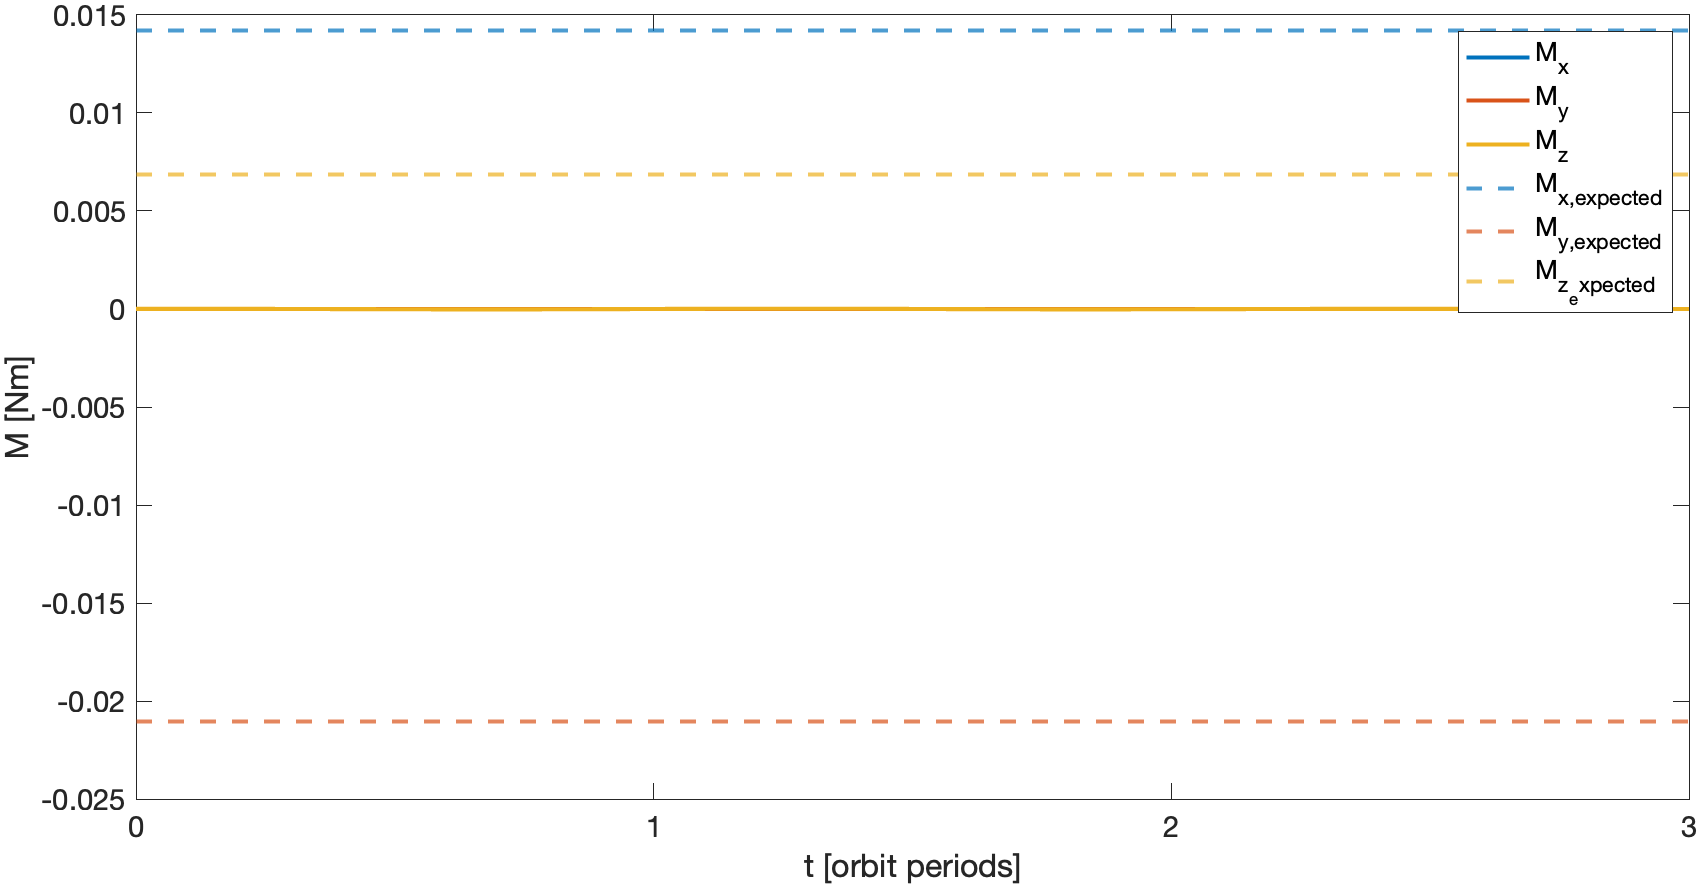
\includegraphics[width = 10cm]{Images/PS4/gravity_torque_RTN_aligned.png}
    \caption{Gravity Gradient Induced Torque Components Represented in Principal Frame Along with Expected Magnitides for Misaligned Torques}
    \label{fig:gravity_gradienet_RTN_aligned}
\end{figure}

\subsubsection{Numerically integrate Euler and Kinematic equations including gravity gradient from arbitrary
initial conditions (e.g., relevant to your project). Plot external torque (3 components w.r.t. time)
and resulting attitude motion (depends on attitude parameterization, add Euler angles for better
geometrical interpretation) over multiple orbits. Comment on results.}

\begin{figure}[H]
    \centering
    \captionsetup{ justification = centering}
    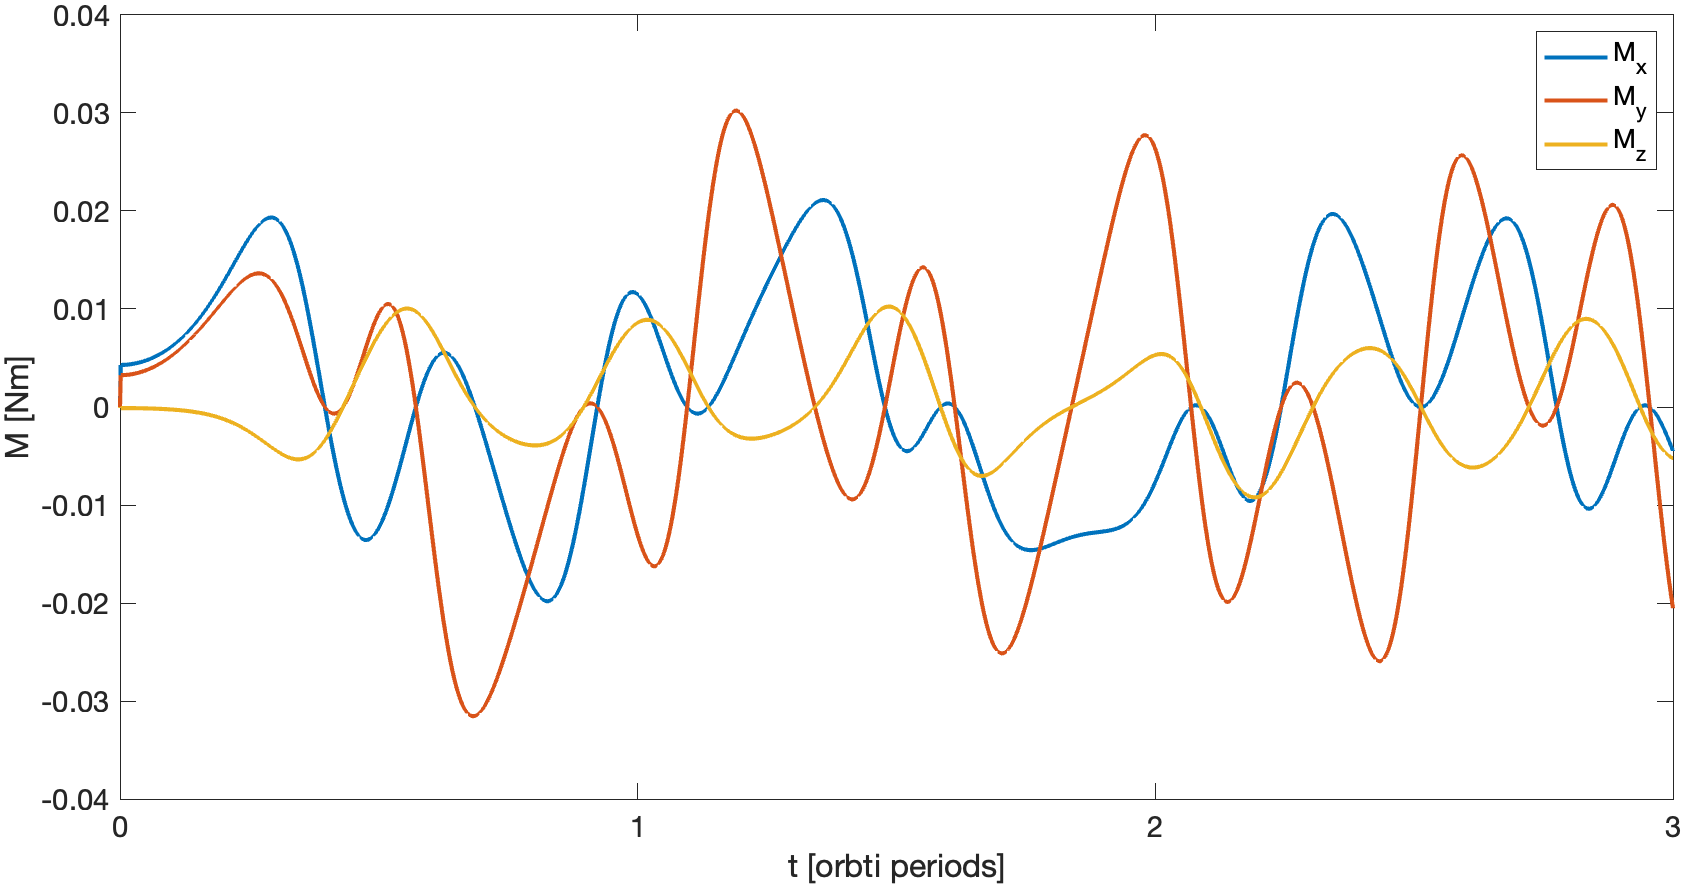
\includegraphics[width = 10cm]{Images/PS4/gravity_torque_mission_aligned.png}
    \caption{Gravity Gradient Induced Torque Components Represented in Principal Frame}
    \label{fig:gravity_gradienet_mission_aligned}
\end{figure}

\begin{figure}[H]
    \centering
    \captionsetup{ justification = centering}
    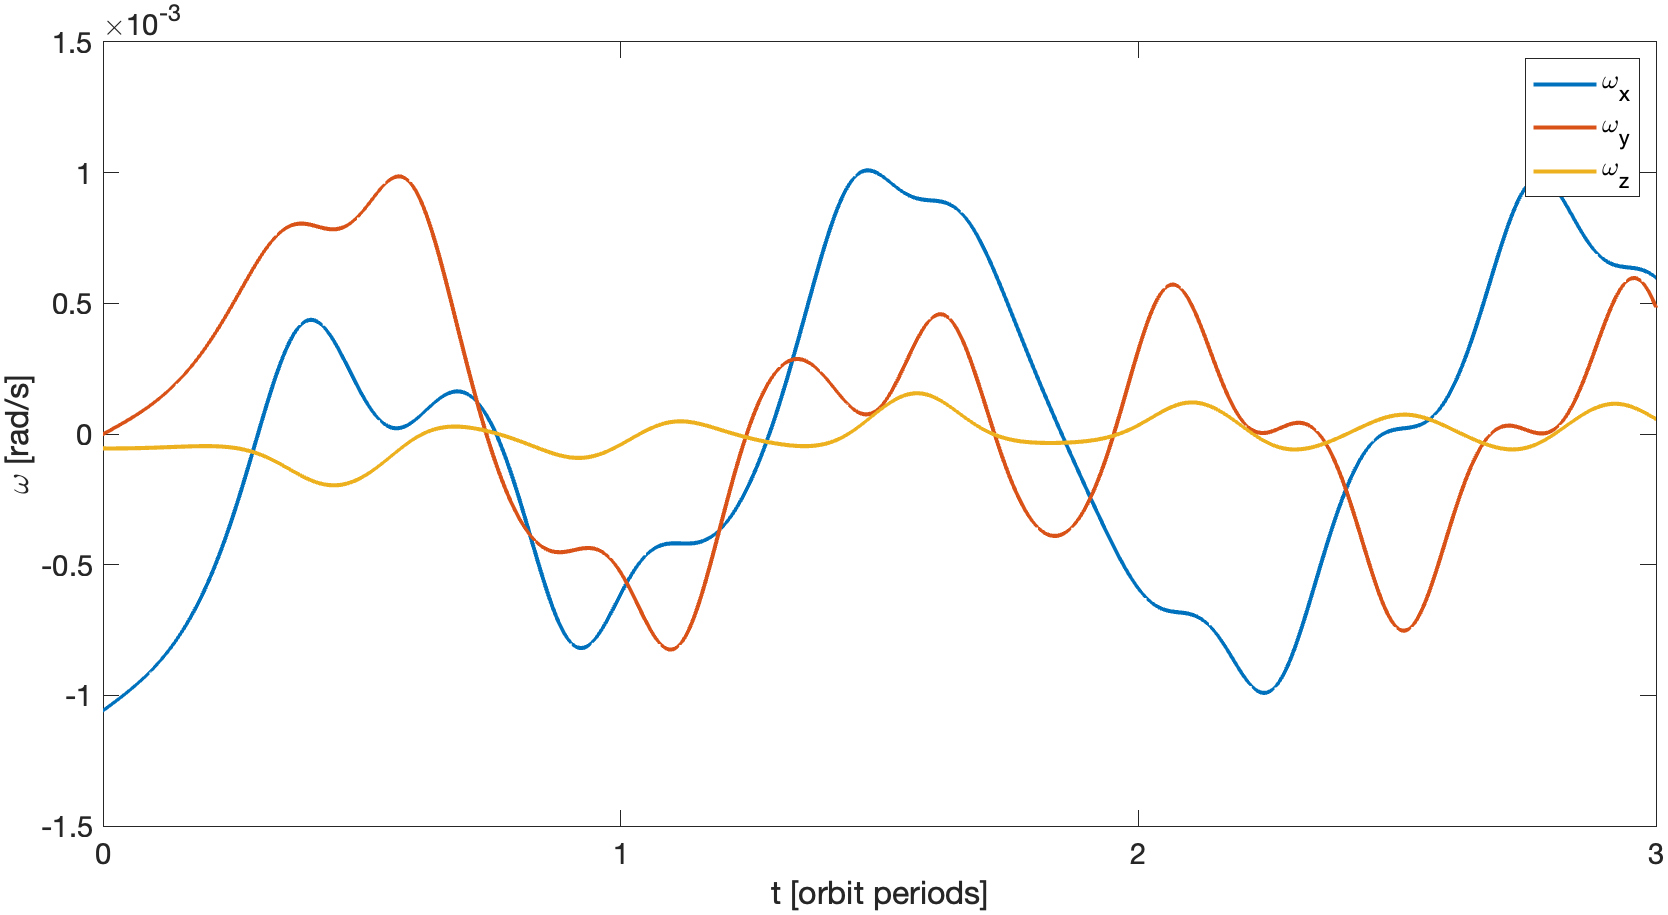
\includegraphics[width = 10cm]{Images/PS4/angular_velocity_under_grav.png}
    \caption{Time History of Angular Velocity Vector Components Expressed in Principal Frame for Mission Aligned Configuration with Gravity Induced Torques}
    \label{fig:grav_mission_velocities}
\end{figure}

\begin{figure}[H]
    \centering
    \captionsetup{justification = centering}
    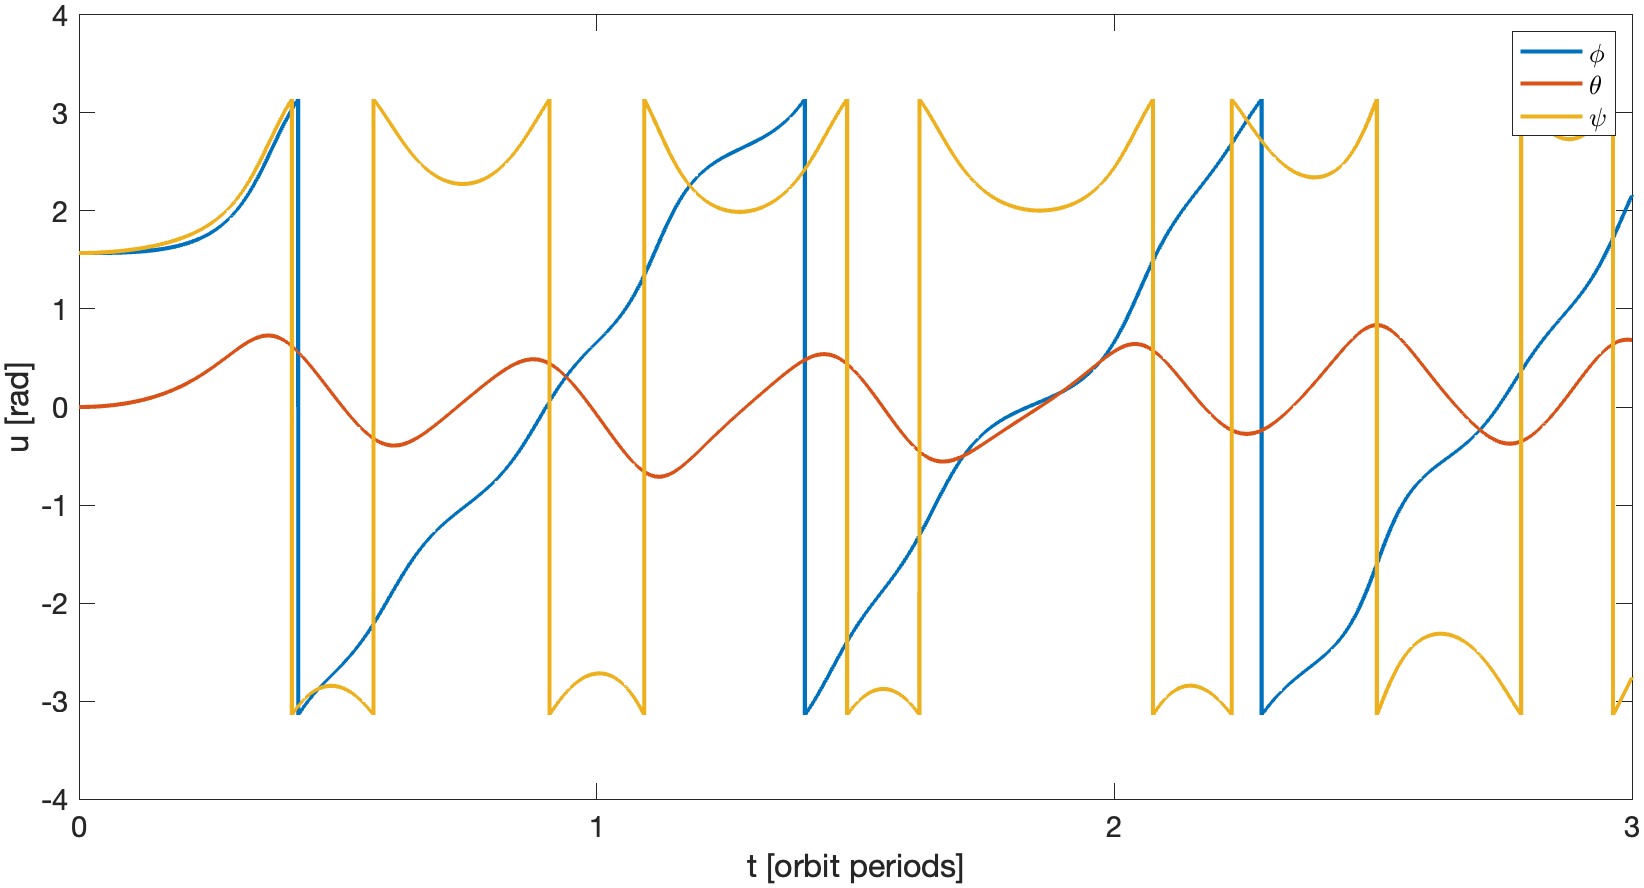
\includegraphics[width = 10cm]{Images/PS4/attitude_under_grav.png}
    \caption{Time History of Perturbed 312 Euler Angles Describing Rotation between RTN and Body Frame for Mission Aligned Configuration with Gravity Induced Torques}
    \label{fig:grav_mission_attitudes}
\end{figure}
